% Options for packages loaded elsewhere
\PassOptionsToPackage{unicode}{hyperref}
\PassOptionsToPackage{hyphens}{url}
\documentclass[
]{article}
\usepackage{xcolor}
\usepackage[margin=1in]{geometry}
\usepackage{amsmath,amssymb}
\setcounter{secnumdepth}{-\maxdimen} % remove section numbering
\usepackage{iftex}
\ifPDFTeX
  \usepackage[T1]{fontenc}
  \usepackage[utf8]{inputenc}
  \usepackage{textcomp} % provide euro and other symbols
\else % if luatex or xetex
  \usepackage{unicode-math} % this also loads fontspec
  \defaultfontfeatures{Scale=MatchLowercase}
  \defaultfontfeatures[\rmfamily]{Ligatures=TeX,Scale=1}
\fi
\usepackage{lmodern}
\ifPDFTeX\else
  % xetex/luatex font selection
\fi
% Use upquote if available, for straight quotes in verbatim environments
\IfFileExists{upquote.sty}{\usepackage{upquote}}{}
\IfFileExists{microtype.sty}{% use microtype if available
  \usepackage[]{microtype}
  \UseMicrotypeSet[protrusion]{basicmath} % disable protrusion for tt fonts
}{}
\makeatletter
\@ifundefined{KOMAClassName}{% if non-KOMA class
  \IfFileExists{parskip.sty}{%
    \usepackage{parskip}
  }{% else
    \setlength{\parindent}{0pt}
    \setlength{\parskip}{6pt plus 2pt minus 1pt}}
}{% if KOMA class
  \KOMAoptions{parskip=half}}
\makeatother
\usepackage{color}
\usepackage{fancyvrb}
\newcommand{\VerbBar}{|}
\newcommand{\VERB}{\Verb[commandchars=\\\{\}]}
\DefineVerbatimEnvironment{Highlighting}{Verbatim}{commandchars=\\\{\}}
% Add ',fontsize=\small' for more characters per line
\usepackage{framed}
\definecolor{shadecolor}{RGB}{248,248,248}
\newenvironment{Shaded}{\begin{snugshade}}{\end{snugshade}}
\newcommand{\AlertTok}[1]{\textcolor[rgb]{0.94,0.16,0.16}{#1}}
\newcommand{\AnnotationTok}[1]{\textcolor[rgb]{0.56,0.35,0.01}{\textbf{\textit{#1}}}}
\newcommand{\AttributeTok}[1]{\textcolor[rgb]{0.13,0.29,0.53}{#1}}
\newcommand{\BaseNTok}[1]{\textcolor[rgb]{0.00,0.00,0.81}{#1}}
\newcommand{\BuiltInTok}[1]{#1}
\newcommand{\CharTok}[1]{\textcolor[rgb]{0.31,0.60,0.02}{#1}}
\newcommand{\CommentTok}[1]{\textcolor[rgb]{0.56,0.35,0.01}{\textit{#1}}}
\newcommand{\CommentVarTok}[1]{\textcolor[rgb]{0.56,0.35,0.01}{\textbf{\textit{#1}}}}
\newcommand{\ConstantTok}[1]{\textcolor[rgb]{0.56,0.35,0.01}{#1}}
\newcommand{\ControlFlowTok}[1]{\textcolor[rgb]{0.13,0.29,0.53}{\textbf{#1}}}
\newcommand{\DataTypeTok}[1]{\textcolor[rgb]{0.13,0.29,0.53}{#1}}
\newcommand{\DecValTok}[1]{\textcolor[rgb]{0.00,0.00,0.81}{#1}}
\newcommand{\DocumentationTok}[1]{\textcolor[rgb]{0.56,0.35,0.01}{\textbf{\textit{#1}}}}
\newcommand{\ErrorTok}[1]{\textcolor[rgb]{0.64,0.00,0.00}{\textbf{#1}}}
\newcommand{\ExtensionTok}[1]{#1}
\newcommand{\FloatTok}[1]{\textcolor[rgb]{0.00,0.00,0.81}{#1}}
\newcommand{\FunctionTok}[1]{\textcolor[rgb]{0.13,0.29,0.53}{\textbf{#1}}}
\newcommand{\ImportTok}[1]{#1}
\newcommand{\InformationTok}[1]{\textcolor[rgb]{0.56,0.35,0.01}{\textbf{\textit{#1}}}}
\newcommand{\KeywordTok}[1]{\textcolor[rgb]{0.13,0.29,0.53}{\textbf{#1}}}
\newcommand{\NormalTok}[1]{#1}
\newcommand{\OperatorTok}[1]{\textcolor[rgb]{0.81,0.36,0.00}{\textbf{#1}}}
\newcommand{\OtherTok}[1]{\textcolor[rgb]{0.56,0.35,0.01}{#1}}
\newcommand{\PreprocessorTok}[1]{\textcolor[rgb]{0.56,0.35,0.01}{\textit{#1}}}
\newcommand{\RegionMarkerTok}[1]{#1}
\newcommand{\SpecialCharTok}[1]{\textcolor[rgb]{0.81,0.36,0.00}{\textbf{#1}}}
\newcommand{\SpecialStringTok}[1]{\textcolor[rgb]{0.31,0.60,0.02}{#1}}
\newcommand{\StringTok}[1]{\textcolor[rgb]{0.31,0.60,0.02}{#1}}
\newcommand{\VariableTok}[1]{\textcolor[rgb]{0.00,0.00,0.00}{#1}}
\newcommand{\VerbatimStringTok}[1]{\textcolor[rgb]{0.31,0.60,0.02}{#1}}
\newcommand{\WarningTok}[1]{\textcolor[rgb]{0.56,0.35,0.01}{\textbf{\textit{#1}}}}
\usepackage{longtable,booktabs,array}
\newcounter{none} % for unnumbered tables
\usepackage{calc} % for calculating minipage widths
% Correct order of tables after \paragraph or \subparagraph
\usepackage{etoolbox}
\makeatletter
\patchcmd\longtable{\par}{\if@noskipsec\mbox{}\fi\par}{}{}
\makeatother
% Allow footnotes in longtable head/foot
\IfFileExists{footnotehyper.sty}{\usepackage{footnotehyper}}{\usepackage{footnote}}
\makesavenoteenv{longtable}
\usepackage{graphicx}
\makeatletter
\newsavebox\pandoc@box
\newcommand*\pandocbounded[1]{% scales image to fit in text height/width
  \sbox\pandoc@box{#1}%
  \Gscale@div\@tempa{\textheight}{\dimexpr\ht\pandoc@box+\dp\pandoc@box\relax}%
  \Gscale@div\@tempb{\linewidth}{\wd\pandoc@box}%
  \ifdim\@tempb\p@<\@tempa\p@\let\@tempa\@tempb\fi% select the smaller of both
  \ifdim\@tempa\p@<\p@\scalebox{\@tempa}{\usebox\pandoc@box}%
  \else\usebox{\pandoc@box}%
  \fi%
}
% Set default figure placement to htbp
\def\fps@figure{htbp}
\makeatother
\setlength{\emergencystretch}{3em} % prevent overfull lines
\providecommand{\tightlist}{%
  \setlength{\itemsep}{0pt}\setlength{\parskip}{0pt}}
\usepackage{bookmark}
\IfFileExists{xurl.sty}{\usepackage{xurl}}{} % add URL line breaks if available
\urlstyle{same}
\hypersetup{
  pdftitle={Mullen TreeFlux Analysis},
  pdfauthor={JM},
  hidelinks,
  pdfcreator={LaTeX via pandoc}}

\title{Mullen TreeFlux Analysis}
\author{JM}
\date{2026-06-30}

\begin{document}
\maketitle

{
\setcounter{tocdepth}{2}
\tableofcontents
}
Welcome to the TEMPEST Flood Tree Greenhouse Gas Flux dataset analysis!

\section{TEMPEST flood dates}\label{tempest-flood-dates}

\begin{Shaded}
\begin{Highlighting}[]
\NormalTok{flood\_date }\OtherTok{\textless{}{-}} \FunctionTok{tribble}\NormalTok{(}\SpecialCharTok{\textasciitilde{}}\NormalTok{Event, }\SpecialCharTok{\textasciitilde{}}\NormalTok{Start, }\SpecialCharTok{\textasciitilde{}}\NormalTok{End,}
                      \StringTok{"T1"}\NormalTok{, }\StringTok{"2022{-}06{-}22"}\NormalTok{, }\StringTok{"2022{-}06{-}22"}\NormalTok{,}
                      \StringTok{"T2"}\NormalTok{, }\StringTok{"2023{-}06{-}06"}\NormalTok{, }\StringTok{"2023{-}06{-}07"}\NormalTok{,}
                      \StringTok{"T3"}\NormalTok{, }\StringTok{"2024{-}06{-}11"}\NormalTok{, }\StringTok{"2024{-}06{-}13"}\NormalTok{)}
\NormalTok{flood\_date}\SpecialCharTok{$}\NormalTok{Start }\OtherTok{\textless{}{-}} \FunctionTok{ymd}\NormalTok{(flood\_date}\SpecialCharTok{$}\NormalTok{Start)}
\NormalTok{flood\_date}\SpecialCharTok{$}\NormalTok{End }\OtherTok{\textless{}{-}} \FunctionTok{ymd}\NormalTok{(flood\_date}\SpecialCharTok{$}\NormalTok{End)}

\NormalTok{knitr}\SpecialCharTok{::}\FunctionTok{kable}\NormalTok{(flood\_date)}
\end{Highlighting}
\end{Shaded}

{\def\LTcaptype{none} % do not increment counter
\begin{longtable}[]{@{}lll@{}}
\toprule\noalign{}
Event & Start & End \\
\midrule\noalign{}
\endhead
\bottomrule\noalign{}
\endlastfoot
T1 & 2022-06-22 & 2022-06-22 \\
T2 & 2023-06-06 & 2023-06-07 \\
T3 & 2024-06-11 & 2024-06-13 \\
\end{longtable}
}

\section{Read data}\label{read-data}

\begin{Shaded}
\begin{Highlighting}[]
\CommentTok{\# Read in data from Apache Parquet file {-}{-}{-}{-}{-}}
\NormalTok{FLUX\_DATA\_FILE }\OtherTok{\textless{}{-}} \StringTok{"tempest\_tree\_ghg\_fluxes.parquet"}
\FunctionTok{message}\NormalTok{(}\StringTok{"Reading "}\NormalTok{, FLUX\_DATA\_FILE)}
\end{Highlighting}
\end{Shaded}

\begin{verbatim}
## Reading tempest_tree_ghg_fluxes.parquet
\end{verbatim}

\begin{Shaded}
\begin{Highlighting}[]
\NormalTok{my\_data }\OtherTok{\textless{}{-}} \FunctionTok{read\_parquet}\NormalTok{(FLUX\_DATA\_FILE)}

\NormalTok{code\_to\_name }\OtherTok{\textless{}{-}} \FunctionTok{c}\NormalTok{(}\AttributeTok{ACRU =} \StringTok{"Red Maple"}\NormalTok{, }\AttributeTok{FAGR =} \StringTok{"Beech"}\NormalTok{, }\AttributeTok{LITU =} \StringTok{"Tulip Poplar"}\NormalTok{)}

\NormalTok{TREE\_MAPPING\_FILE }\OtherTok{\textless{}{-}} \StringTok{"ancillary\_data/sapflow\_tree\_mapping.csv"}
\FunctionTok{message}\NormalTok{(}\StringTok{"Reading "}\NormalTok{, TREE\_MAPPING\_FILE)}
\end{Highlighting}
\end{Shaded}

\begin{verbatim}
## Reading ancillary_data/sapflow_tree_mapping.csv
\end{verbatim}

\begin{Shaded}
\begin{Highlighting}[]
\NormalTok{tree\_map }\OtherTok{\textless{}{-}} \FunctionTok{read.csv}\NormalTok{(TREE\_MAPPING\_FILE,}
                     \AttributeTok{stringsAsFactors =} \ConstantTok{FALSE}\NormalTok{) }\SpecialCharTok{\%\textgreater{}\%}
  \FunctionTok{mutate}\NormalTok{(}\FunctionTok{across}\NormalTok{(}\FunctionTok{where}\NormalTok{(is.character), trimws)) }\SpecialCharTok{\%\textgreater{}\%}
  \FunctionTok{transmute}\NormalTok{(}\AttributeTok{ID =}\NormalTok{ Sapflux\_ID,}
            \AttributeTok{Species\_from\_map =} \FunctionTok{unname}\NormalTok{(code\_to\_name[Species\_Code])) }\SpecialCharTok{\%\textgreater{}\%}
  \FunctionTok{distinct}\NormalTok{(ID, }\AttributeTok{.keep\_all =} \ConstantTok{TRUE}\NormalTok{)}

\NormalTok{my\_data }\OtherTok{\textless{}{-}}\NormalTok{ my\_data }\SpecialCharTok{\%\textgreater{}\%}
  \FunctionTok{left\_join}\NormalTok{(tree\_map, }\AttributeTok{by =} \StringTok{"ID"}\NormalTok{) }\SpecialCharTok{\%\textgreater{}\%}
  \FunctionTok{mutate}\NormalTok{(}\AttributeTok{Species =} \FunctionTok{coalesce}\NormalTok{(Species, Species\_from\_map)) }\SpecialCharTok{\%\textgreater{}\%}
  \FunctionTok{select}\NormalTok{(}\SpecialCharTok{{-}}\NormalTok{Species\_from\_map)}

\FunctionTok{message}\NormalTok{(}\StringTok{"Trees with NA species: "}\NormalTok{, }\FunctionTok{sum}\NormalTok{(}\FunctionTok{is.na}\NormalTok{(my\_data}\SpecialCharTok{$}\NormalTok{Species)))}
\end{Highlighting}
\end{Shaded}

\begin{verbatim}
## Trees with NA species: 0
\end{verbatim}

\section{Prep Soil Temp Data}\label{prep-soil-temp-data}

\begin{Shaded}
\begin{Highlighting}[]
\FunctionTok{read\_L2\_variable}\NormalTok{(}\AttributeTok{variable =} \StringTok{"soil{-}temp{-}5cm"}\NormalTok{, }\AttributeTok{path =} \StringTok{"Sensor\_Data/"}\NormalTok{, }\AttributeTok{quiet=}\ConstantTok{TRUE}\NormalTok{)}
\end{Highlighting}
\end{Shaded}

\subsection{Take daily avg}\label{take-daily-avg}

\begin{Shaded}
\begin{Highlighting}[]
\NormalTok{soil\_temp\_data }\OtherTok{\textless{}{-}} \FunctionTok{read\_L2\_variable}\NormalTok{(}\AttributeTok{variable =} \StringTok{"soil{-}temp{-}5cm"}\NormalTok{,}
                                   \AttributeTok{path =} \StringTok{"Sensor\_Data/"}\NormalTok{, }\AttributeTok{quiet =} \ConstantTok{TRUE}\NormalTok{)}
\NormalTok{soil\_temp\_daily }\OtherTok{\textless{}{-}}\NormalTok{ soil\_temp\_data }\SpecialCharTok{\%\textgreater{}\%}
  \FunctionTok{mutate}\NormalTok{(}
\CommentTok{\#    TIMESTAMP = as.POSIXct(TIMESTAMP),}
    \AttributeTok{Date =} \FunctionTok{as.Date}\NormalTok{(TIMESTAMP),}
    \AttributeTok{Value =} \FunctionTok{as.numeric}\NormalTok{(Value) ) }\SpecialCharTok{\%\textgreater{}\%}
  \FunctionTok{filter}\NormalTok{(}\SpecialCharTok{!}\FunctionTok{is.na}\NormalTok{(Value)) }\SpecialCharTok{\%\textgreater{}\%}  
  \FunctionTok{group\_by}\NormalTok{(Site, Plot, Date) }\SpecialCharTok{\%\textgreater{}\%}
  \FunctionTok{summarise}\NormalTok{(}
    \AttributeTok{soil\_temp\_daily\_mean =} \FunctionTok{mean}\NormalTok{(Value),}
    \AttributeTok{n =} \FunctionTok{n}\NormalTok{(),}
    \CommentTok{\# }\AlertTok{TODO}\CommentTok{: explain this next step (what\textquotesingle{}s 480?)}
    \AttributeTok{coverage =}\NormalTok{ n }\SpecialCharTok{/} \DecValTok{480}\NormalTok{,      }
    \AttributeTok{.groups =} \StringTok{"drop"}\NormalTok{  )}
\FunctionTok{print}\NormalTok{(soil\_temp\_daily)}
\end{Highlighting}
\end{Shaded}

\begin{verbatim}
## # A tibble: 6,020 x 6
##    Site  Plot  Date       soil_temp_daily_mean     n coverage
##    <chr> <chr> <date>                    <dbl> <int>    <dbl>
##  1 TMP   C     2020-05-05                12.7     37   0.0771
##  2 TMP   C     2020-05-06                11.9     96   0.2   
##  3 TMP   C     2020-05-07                11.4     96   0.2   
##  4 TMP   C     2020-05-08                11.9     96   0.2   
##  5 TMP   C     2020-05-09                 9.68    96   0.2   
##  6 TMP   C     2020-05-10                 9.76    96   0.2   
##  7 TMP   C     2020-05-11                11.1     96   0.2   
##  8 TMP   C     2020-05-12                10.6     96   0.2   
##  9 TMP   C     2020-05-13                11.3     96   0.2   
## 10 TMP   C     2020-05-14                12.2     96   0.2   
## # i 6,010 more rows
\end{verbatim}

\subsection{Graphs of Soil Temp Data (Daily averages over
time)}\label{graphs-of-soil-temp-data-daily-averages-over-time}

\begin{Shaded}
\begin{Highlighting}[]
\FunctionTok{ggplot}\NormalTok{(soil\_temp\_daily,}\FunctionTok{aes}\NormalTok{(}\AttributeTok{x =}\NormalTok{ Date, }\AttributeTok{y =}\NormalTok{ soil\_temp\_daily\_mean,}
\AttributeTok{color =}\NormalTok{ Plot, }\AttributeTok{group =}\NormalTok{ Plot)) }\SpecialCharTok{+} \FunctionTok{geom\_line}\NormalTok{(}\AttributeTok{alpha =} \FloatTok{0.7}\NormalTok{) }\SpecialCharTok{+} \FunctionTok{facet\_wrap}\NormalTok{(}\SpecialCharTok{\textasciitilde{}}\NormalTok{ Site) }\SpecialCharTok{+}
\FunctionTok{labs}\NormalTok{( }\AttributeTok{title =} \StringTok{"Daily Mean Soil Temperature by Plot"}\NormalTok{,}
   \AttributeTok{x =} \StringTok{"Date"}\NormalTok{,}
   \AttributeTok{y =} \StringTok{"Soil Temperature (°C)"}\NormalTok{ ) }
\end{Highlighting}
\end{Shaded}

\pandocbounded{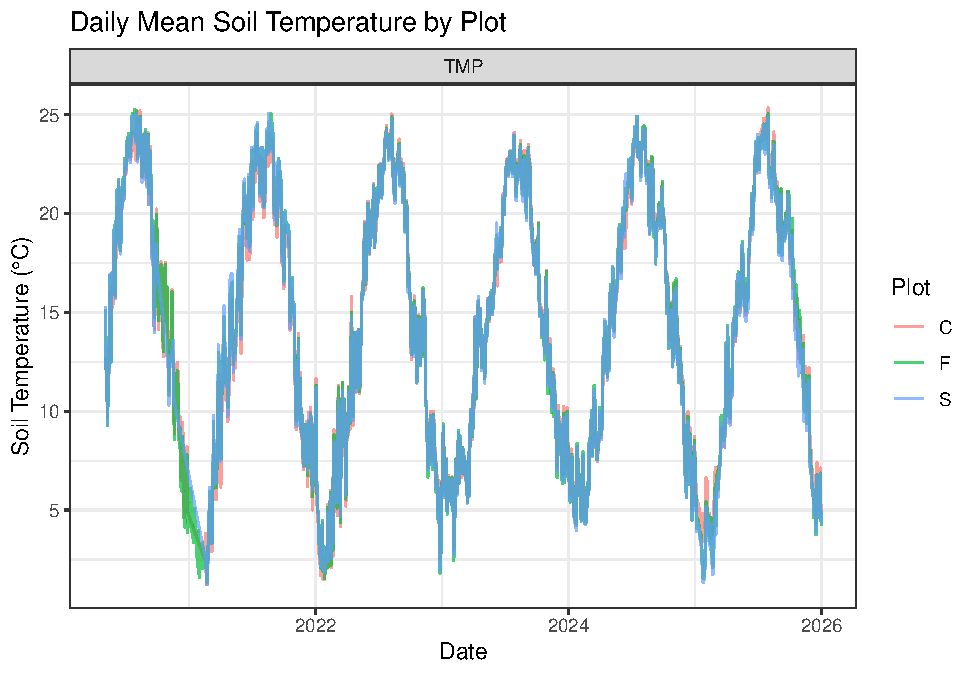
\includegraphics[keepaspectratio]{Mullen_TreeFlux_Analysis_files/Mullen_TreeFlux_Analysis_files/figure-latex/unnamed-chunk-3-1.pdf}}

\subsection{Matching the plot names from tree flux and soil
temp}\label{matching-the-plot-names-from-tree-flux-and-soil-temp}

\begin{Shaded}
\begin{Highlighting}[]
\NormalTok{soil\_temp\_daily }\OtherTok{\textless{}{-}}\NormalTok{ soil\_temp\_daily }\SpecialCharTok{\%\textgreater{}\%}
  \FunctionTok{mutate}\NormalTok{( }\AttributeTok{Plot =} \FunctionTok{recode}\NormalTok{(Plot,}
         \StringTok{"C"} \OtherTok{=} \StringTok{"Control"}\NormalTok{,}
         \StringTok{"F"} \OtherTok{=} \StringTok{"Freshwater"}\NormalTok{,}
         \StringTok{"S"} \OtherTok{=} \StringTok{"Seawater"}\NormalTok{ )  )}
\end{Highlighting}
\end{Shaded}

\subsection{Joining datasets}\label{joining-datasets}

\begin{Shaded}
\begin{Highlighting}[]
\NormalTok{my\_data }\OtherTok{\textless{}{-}}\NormalTok{ my\_data }\SpecialCharTok{\%\textgreater{}\%}
  \FunctionTok{left\_join}\NormalTok{(}
\NormalTok{     soil\_temp\_daily }\SpecialCharTok{\%\textgreater{}\%}
    \FunctionTok{select}\NormalTok{(Plot, Date, soil\_temp\_daily\_mean),}
    \AttributeTok{by =} \FunctionTok{c}\NormalTok{(}\StringTok{"Plot"}\NormalTok{, }\StringTok{"Date"}\NormalTok{))}
\end{Highlighting}
\end{Shaded}

\section{Numerical summaries -----}\label{numerical-summaries}

print(my\_data) \# BBL: print summary of fluxes? A table with mean, min,
max and date ranges

\begin{Shaded}
\begin{Highlighting}[]
\NormalTok{ my\_data }\SpecialCharTok{\%\textgreater{}\%}
   \FunctionTok{ggplot}\NormalTok{(}\FunctionTok{aes}\NormalTok{( }\AttributeTok{x =}\NormalTok{ Year, }\AttributeTok{y =}\NormalTok{ CH4\_lin\_flux.estimate, }\AttributeTok{color =}\NormalTok{ Plot )) }\SpecialCharTok{+}
   \FunctionTok{geom\_point}\NormalTok{(}\AttributeTok{alpha =} \FloatTok{0.6}\NormalTok{) }\SpecialCharTok{+}
   \FunctionTok{facet\_wrap}\NormalTok{(}\SpecialCharTok{\textasciitilde{}}\NormalTok{ Species) }\SpecialCharTok{+}
   \FunctionTok{labs}\NormalTok{( }\AttributeTok{title =} \StringTok{"CH4 Flux by Species (2021–2025)"}\NormalTok{ )}
\end{Highlighting}
\end{Shaded}

\pandocbounded{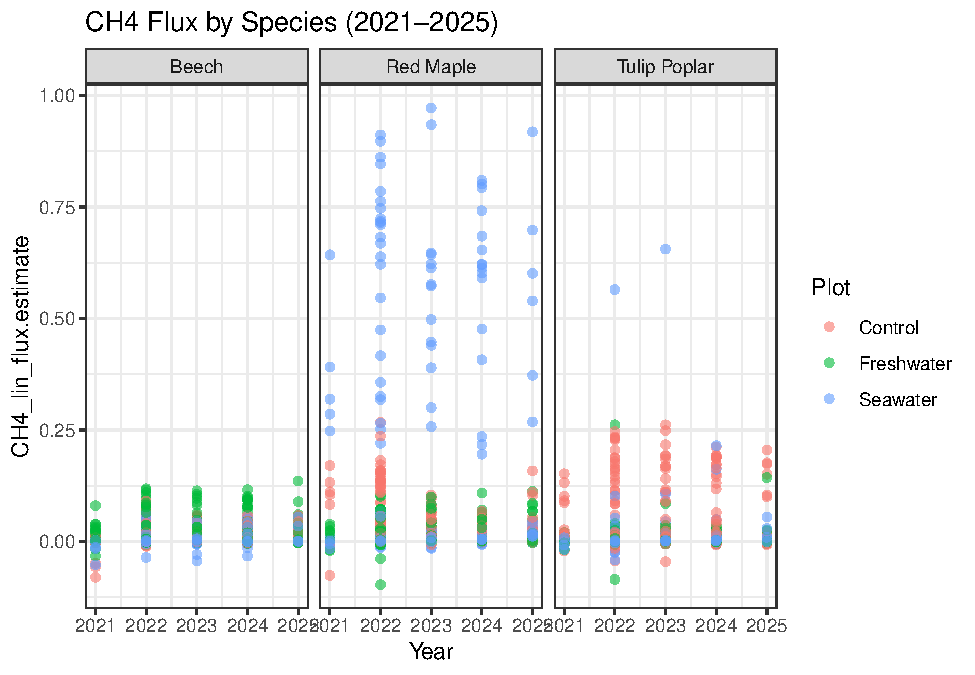
\includegraphics[keepaspectratio]{Mullen_TreeFlux_Analysis_files/Mullen_TreeFlux_Analysis_files/figure-latex/unnamed-chunk-6-1.pdf}}

\begin{Shaded}
\begin{Highlighting}[]
\NormalTok{my\_data }\SpecialCharTok{\%\textgreater{}\%}
  \FunctionTok{ggplot}\NormalTok{(}\FunctionTok{aes}\NormalTok{( }\AttributeTok{x =}\NormalTok{ Year, }\AttributeTok{y =}\NormalTok{ CO2\_lin\_flux.estimate, }\AttributeTok{color =}\NormalTok{ Plot )) }\SpecialCharTok{+}
  \FunctionTok{geom\_point}\NormalTok{(}\AttributeTok{alpha =} \FloatTok{0.6}\NormalTok{) }\SpecialCharTok{+}
  \FunctionTok{facet\_wrap}\NormalTok{(}\SpecialCharTok{\textasciitilde{}}\NormalTok{ Species) }\SpecialCharTok{+}
  \FunctionTok{labs}\NormalTok{( }\AttributeTok{title =} \StringTok{"CO2 Flux by Species (2021–2025)"}\NormalTok{, }\AttributeTok{y =} \StringTok{"CO2 Flux"}\NormalTok{ )}
\end{Highlighting}
\end{Shaded}

\pandocbounded{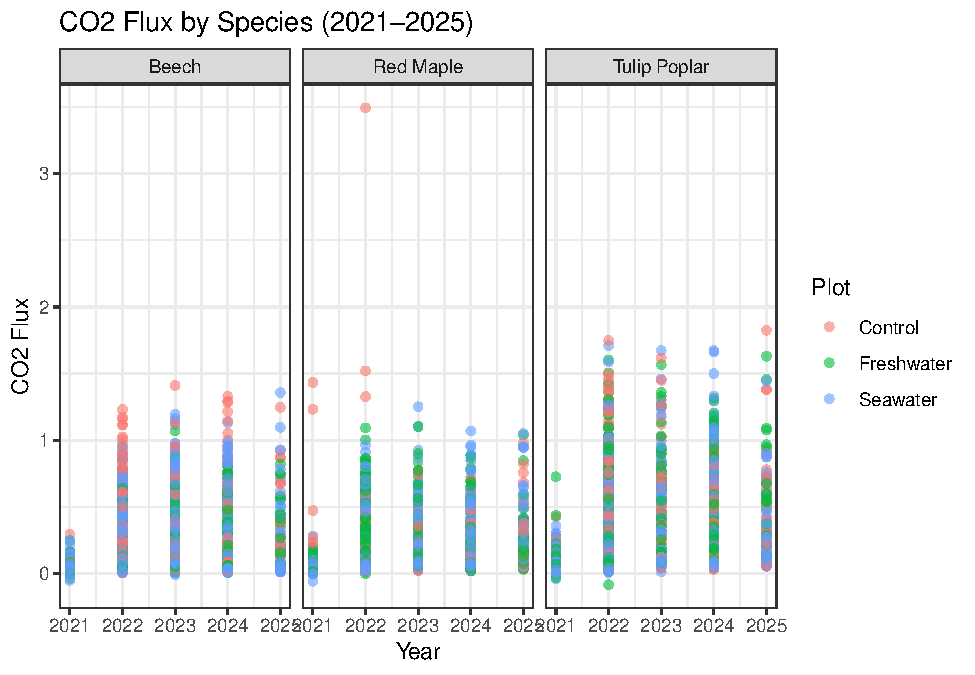
\includegraphics[keepaspectratio]{Mullen_TreeFlux_Analysis_files/Mullen_TreeFlux_Analysis_files/figure-latex/unnamed-chunk-6-2.pdf}}

\section{Numerical summaries}\label{numerical-summaries-1}

\begin{Shaded}
\begin{Highlighting}[]
\FunctionTok{print}\NormalTok{(my\_data)}
\end{Highlighting}
\end{Shaded}

\begin{verbatim}
## # A tibble: 3,361 x 13
## # Groups:   Year, Date, Plot, Timepoint, Species, ID [3,361]
##     Year Date       Plot       Timepoint Species     ID    CO2_lin_flux.estimate
##    <dbl> <date>     <chr>      <chr>     <chr>       <chr>                 <dbl>
##  1  2021 2021-10-08 Control    (none)    Tulip Popl~ C1                   0.425 
##  2  2021 2021-10-08 Control    (none)    Red Maple   C10                  0.227 
##  3  2021 2021-10-08 Control    (none)    Red Maple   C12                  0.0817
##  4  2021 2021-10-08 Control    (none)    Beech       C14                  0.293 
##  5  2021 2021-10-08 Control    (none)    Beech       C16                  0.0628
##  6  2021 2021-10-08 Control    (none)    Beech       C17                  0.139 
##  7  2021 2021-10-08 Control    (none)    Tulip Popl~ C2                   0.228 
##  8  2021 2021-10-08 Control    (none)    Tulip Popl~ C6                   0.181 
##  9  2021 2021-10-08 Control    (none)    Red Maple   C8                   1.43  
## 10  2021 2021-10-08 Freshwater (none)    Tulip Popl~ F1                   0.276 
## # i 3,351 more rows
## # i 6 more variables: CO2_lin_r.squared <dbl>, CO2_rob_flux.estimate <dbl>,
## #   CH4_lin_flux.estimate <dbl>, CH4_lin_r.squared <dbl>,
## #   CH4_rob_flux.estimate <dbl>, soil_temp_daily_mean <dbl>
\end{verbatim}

\begin{Shaded}
\begin{Highlighting}[]
\CommentTok{\# BBL: print summary of fluxes? A table with mean, min, max and date ranges}
\end{Highlighting}
\end{Shaded}

\section{Plots}\label{plots}

\subsubsection{Initial visualizations of Raw
Data}\label{initial-visualizations-of-raw-data}

\subsection{Overall data, by species}\label{overall-data-by-species}

\begin{Shaded}
\begin{Highlighting}[]
\NormalTok{my\_data }\SpecialCharTok{\%\textgreater{}\%}
  \FunctionTok{ggplot}\NormalTok{(}\FunctionTok{aes}\NormalTok{( }\AttributeTok{x =}\NormalTok{ Year, }\AttributeTok{y =}\NormalTok{ CH4\_lin\_flux.estimate, }\AttributeTok{color =}\NormalTok{ Plot )) }\SpecialCharTok{+}
  \FunctionTok{geom\_point}\NormalTok{(}\AttributeTok{alpha =} \FloatTok{0.6}\NormalTok{) }\SpecialCharTok{+}
  \FunctionTok{facet\_wrap}\NormalTok{(}\SpecialCharTok{\textasciitilde{}}\NormalTok{ Species) }\SpecialCharTok{+}
  \FunctionTok{labs}\NormalTok{( }\AttributeTok{title =} \StringTok{"CH4 Flux by Species (2021–2025)"}\NormalTok{ )}
\end{Highlighting}
\end{Shaded}

\pandocbounded{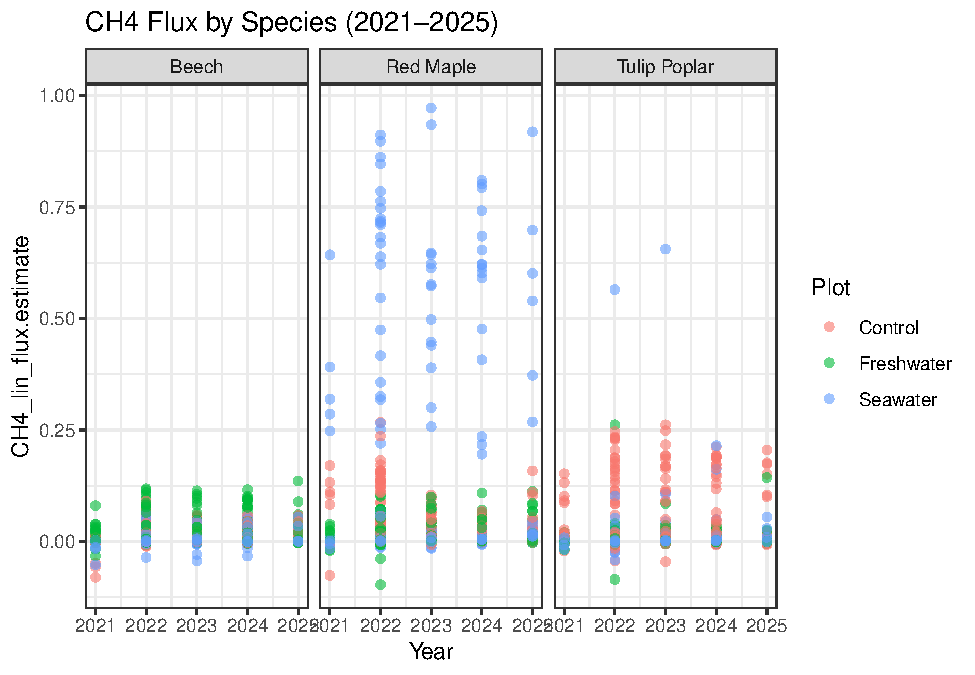
\includegraphics[keepaspectratio]{Mullen_TreeFlux_Analysis_files/Mullen_TreeFlux_Analysis_files/figure-latex/overall-by-species-1.pdf}}

\begin{Shaded}
\begin{Highlighting}[]
\NormalTok{my\_data }\SpecialCharTok{\%\textgreater{}\%}
  \FunctionTok{ggplot}\NormalTok{(}\FunctionTok{aes}\NormalTok{( }\AttributeTok{x =}\NormalTok{ Year, }\AttributeTok{y =}\NormalTok{ CO2\_lin\_flux.estimate, }\AttributeTok{color =}\NormalTok{ Plot )) }\SpecialCharTok{+}
  \FunctionTok{geom\_point}\NormalTok{(}\AttributeTok{alpha =} \FloatTok{0.6}\NormalTok{) }\SpecialCharTok{+}
  \FunctionTok{facet\_wrap}\NormalTok{(}\SpecialCharTok{\textasciitilde{}}\NormalTok{ Species) }\SpecialCharTok{+}
  \FunctionTok{labs}\NormalTok{( }\AttributeTok{title =} \StringTok{"CO2 Flux by Species (2021–2025)"}\NormalTok{, }\AttributeTok{y =} \StringTok{"CO2 Flux"}\NormalTok{ )}
\end{Highlighting}
\end{Shaded}

\pandocbounded{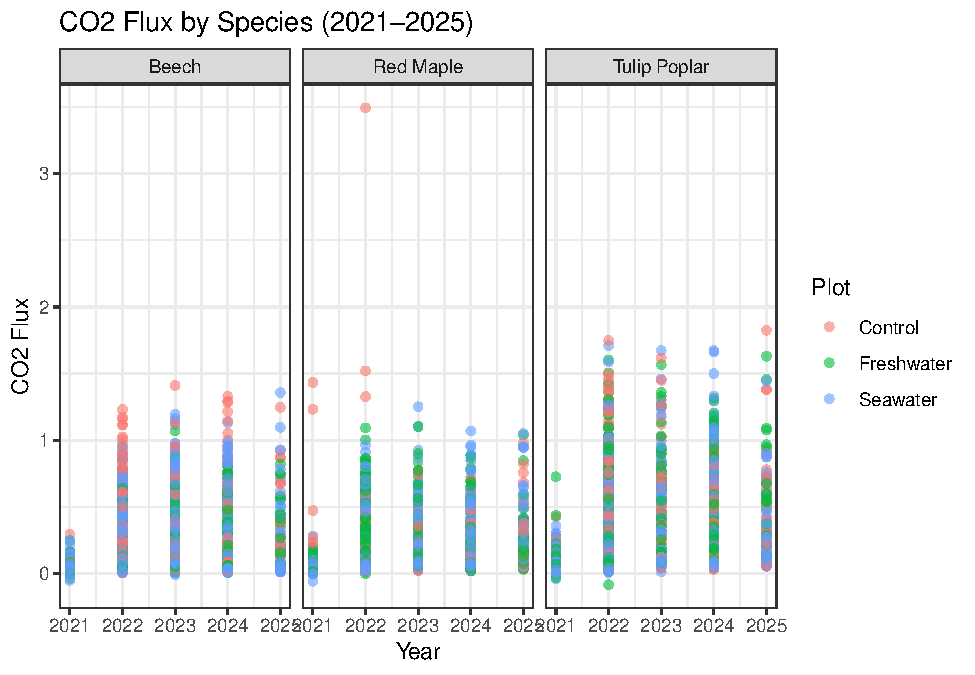
\includegraphics[keepaspectratio]{Mullen_TreeFlux_Analysis_files/Mullen_TreeFlux_Analysis_files/figure-latex/overall-by-species-2.pdf}}

\subsection{Flux ranges by species}\label{flux-ranges-by-species}

\begin{Shaded}
\begin{Highlighting}[]
\CommentTok{\# Overall flux range (using boxplot) for each gas, by tree species}
\FunctionTok{ggplot}\NormalTok{(my\_data,}\FunctionTok{aes}\NormalTok{(}\AttributeTok{x =}\NormalTok{ Species, }\AttributeTok{y =}\NormalTok{ CH4\_lin\_flux.estimate, }\AttributeTok{fill =}\NormalTok{ Plot)) }\SpecialCharTok{+}
  \FunctionTok{geom\_boxplot}\NormalTok{() }\SpecialCharTok{+}
  \FunctionTok{theme\_bw}\NormalTok{() }\SpecialCharTok{+}
  \FunctionTok{theme}\NormalTok{(}\AttributeTok{axis.text.x =} \FunctionTok{element\_text}\NormalTok{(}\AttributeTok{angle =} \DecValTok{45}\NormalTok{, }\AttributeTok{hjust =} \DecValTok{1}\NormalTok{))}
\end{Highlighting}
\end{Shaded}

\pandocbounded{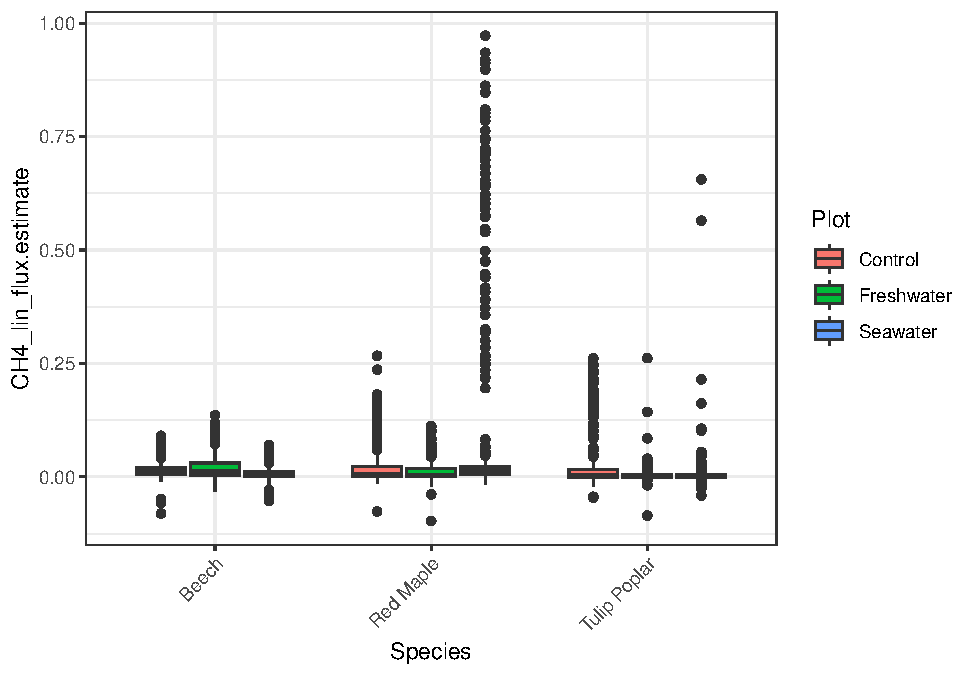
\includegraphics[keepaspectratio]{Mullen_TreeFlux_Analysis_files/Mullen_TreeFlux_Analysis_files/figure-latex/flux-ranges-1.pdf}}

\begin{Shaded}
\begin{Highlighting}[]
\FunctionTok{ggplot}\NormalTok{(my\_data, }\FunctionTok{aes}\NormalTok{(}\AttributeTok{x =}\NormalTok{ Species,  }\AttributeTok{y =}\NormalTok{ CO2\_lin\_flux.estimate, }\AttributeTok{fill =}\NormalTok{ Plot)) }\SpecialCharTok{+}
  \FunctionTok{geom\_boxplot}\NormalTok{() }\SpecialCharTok{+}
  \FunctionTok{theme\_bw}\NormalTok{() }\SpecialCharTok{+}
  \FunctionTok{theme}\NormalTok{(}\AttributeTok{axis.text.x =} \FunctionTok{element\_text}\NormalTok{(}\AttributeTok{angle =} \DecValTok{45}\NormalTok{, }\AttributeTok{hjust =} \DecValTok{1}\NormalTok{))}
\end{Highlighting}
\end{Shaded}

\pandocbounded{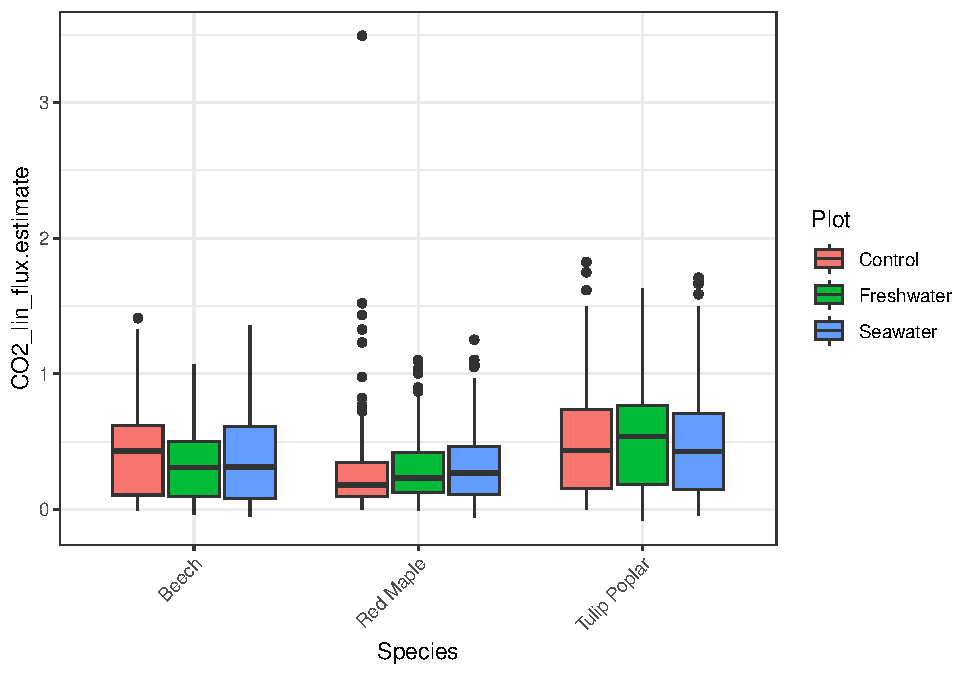
\includegraphics[keepaspectratio]{Mullen_TreeFlux_Analysis_files/Mullen_TreeFlux_Analysis_files/figure-latex/flux-ranges-2.pdf}}

\subsection{Spaghetti plots of Raw
Data}\label{spaghetti-plots-of-raw-data}

\begin{Shaded}
\begin{Highlighting}[]
\FunctionTok{ggplot}\NormalTok{(my\_data, }\FunctionTok{aes}\NormalTok{(}\AttributeTok{x =}\NormalTok{ Date, }\AttributeTok{y =}\NormalTok{ CH4\_lin\_flux.estimate,}
                    \AttributeTok{group =}\NormalTok{ ID, }\AttributeTok{color =}\NormalTok{ Plot)) }\SpecialCharTok{+}
  \FunctionTok{geom\_line}\NormalTok{(}\AttributeTok{alpha =} \FloatTok{0.2}\NormalTok{) }\SpecialCharTok{+}
  \FunctionTok{facet\_wrap}\NormalTok{(}\SpecialCharTok{\textasciitilde{}}\NormalTok{ Species) }\SpecialCharTok{+}
  \FunctionTok{labs}\NormalTok{(}\AttributeTok{title =} \StringTok{"CH4 Flux Over Time by Species and Plot"}\NormalTok{,}
       \AttributeTok{x =} \StringTok{"Date"}\NormalTok{,}
       \AttributeTok{y =} \StringTok{"CH4 Flux"}\NormalTok{)}
\end{Highlighting}
\end{Shaded}

\pandocbounded{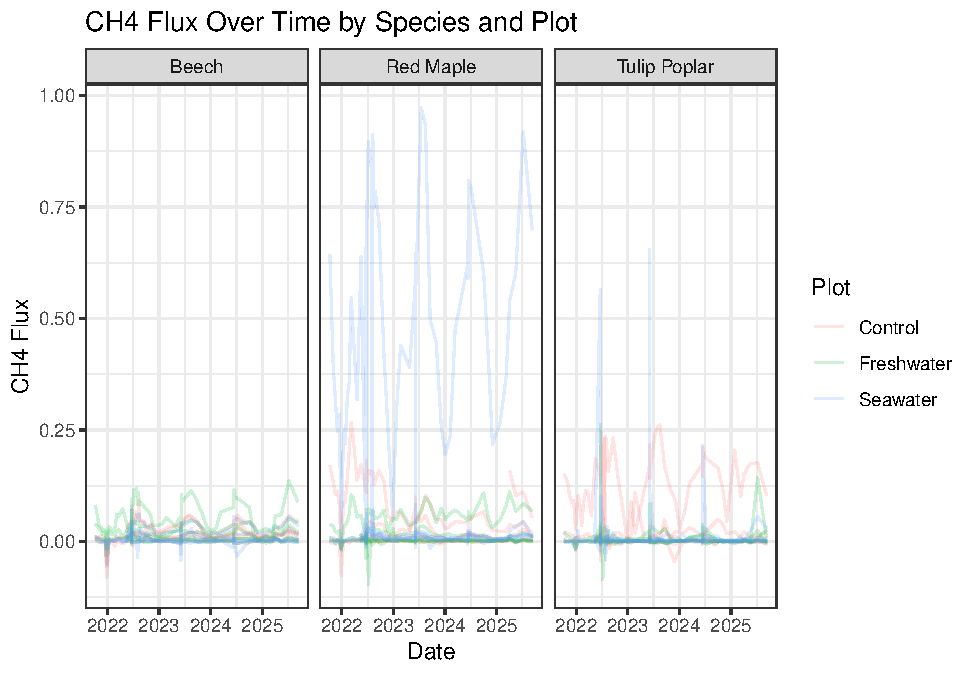
\includegraphics[keepaspectratio]{Mullen_TreeFlux_Analysis_files/Mullen_TreeFlux_Analysis_files/figure-latex/unnamed-chunk-7-1.pdf}}

\begin{Shaded}
\begin{Highlighting}[]
\FunctionTok{ggplot}\NormalTok{(my\_data, }\FunctionTok{aes}\NormalTok{(}\AttributeTok{x =}\NormalTok{ Date,}
                    \AttributeTok{y =}\NormalTok{ CO2\_lin\_flux.estimate,}
                    \AttributeTok{group =}\NormalTok{ ID,}
                    \AttributeTok{color =}\NormalTok{ Plot)) }\SpecialCharTok{+}
  \FunctionTok{geom\_line}\NormalTok{(}\AttributeTok{alpha =} \FloatTok{0.2}\NormalTok{) }\SpecialCharTok{+}
  \FunctionTok{facet\_wrap}\NormalTok{(}\SpecialCharTok{\textasciitilde{}}\NormalTok{ Species) }\SpecialCharTok{+}
  \FunctionTok{labs}\NormalTok{(}
    \AttributeTok{title =} \StringTok{"CO2 Flux Over Time by Species and Plot"}\NormalTok{,}
    \AttributeTok{x =} \StringTok{"Date"}\NormalTok{,}
    \AttributeTok{y =} \StringTok{"CO2 Flux"}\NormalTok{ )}
\end{Highlighting}
\end{Shaded}

\pandocbounded{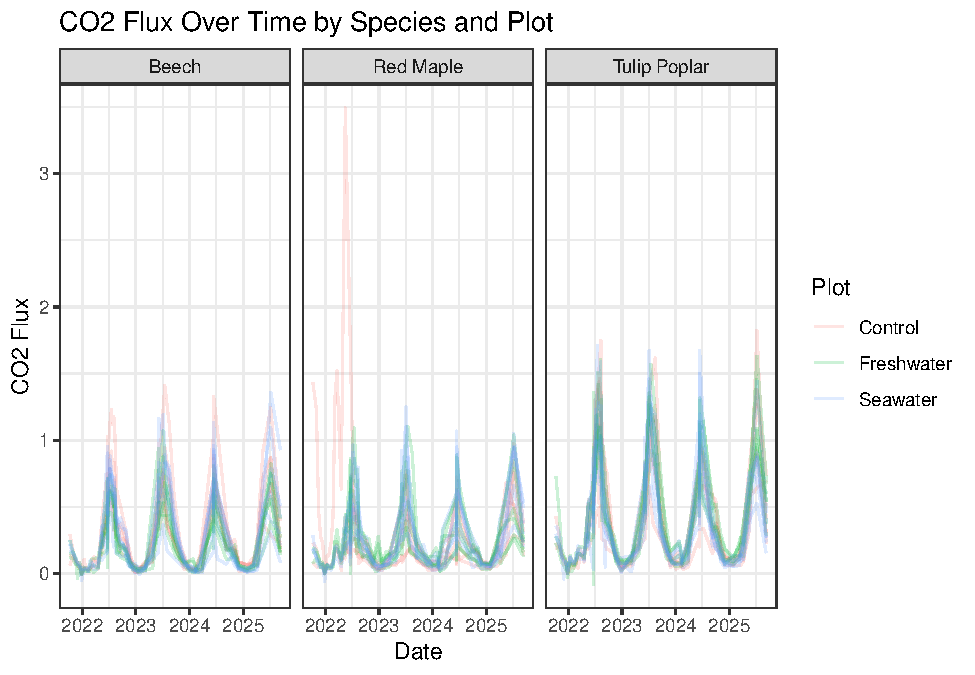
\includegraphics[keepaspectratio]{Mullen_TreeFlux_Analysis_files/Mullen_TreeFlux_Analysis_files/figure-latex/unnamed-chunk-7-2.pdf}}

\subsection{Heat Maps of of Raw Data}\label{heat-maps-of-of-raw-data}

\begin{Shaded}
\begin{Highlighting}[]
\NormalTok{heat\_data\_CH4 }\OtherTok{\textless{}{-}}\NormalTok{ my\_data }\SpecialCharTok{\%\textgreater{}\%}
  \FunctionTok{group\_by}\NormalTok{(Species, Year) }\SpecialCharTok{\%\textgreater{}\%}
  \FunctionTok{summarize}\NormalTok{(}
    \AttributeTok{mean\_flux =} \FunctionTok{mean}\NormalTok{(CH4\_lin\_flux.estimate, }\AttributeTok{na.rm =} \ConstantTok{TRUE}\NormalTok{),}
    \AttributeTok{.groups =} \StringTok{"drop"}\NormalTok{ )}
\FunctionTok{ggplot}\NormalTok{(heat\_data\_CH4, }\FunctionTok{aes}\NormalTok{(}\AttributeTok{x =}\NormalTok{ Year, }\AttributeTok{y =}\NormalTok{ Species, }\AttributeTok{fill =}\NormalTok{ mean\_flux)) }\SpecialCharTok{+}
  \FunctionTok{geom\_tile}\NormalTok{() }\SpecialCharTok{+}
  \FunctionTok{scale\_fill\_viridis\_c}\NormalTok{() }\SpecialCharTok{+}
  \FunctionTok{labs}\NormalTok{( }\AttributeTok{title =} \StringTok{"Mean CH4 Flux by Species and Year"}\NormalTok{, }\AttributeTok{x =} \StringTok{"Year"}\NormalTok{, }\AttributeTok{y =} \StringTok{"Species"}\NormalTok{,}
        \AttributeTok{fill =} \StringTok{"Mean CH4 Flux"}\NormalTok{) }\SpecialCharTok{+} \FunctionTok{theme\_minimal}\NormalTok{()}
\end{Highlighting}
\end{Shaded}

\pandocbounded{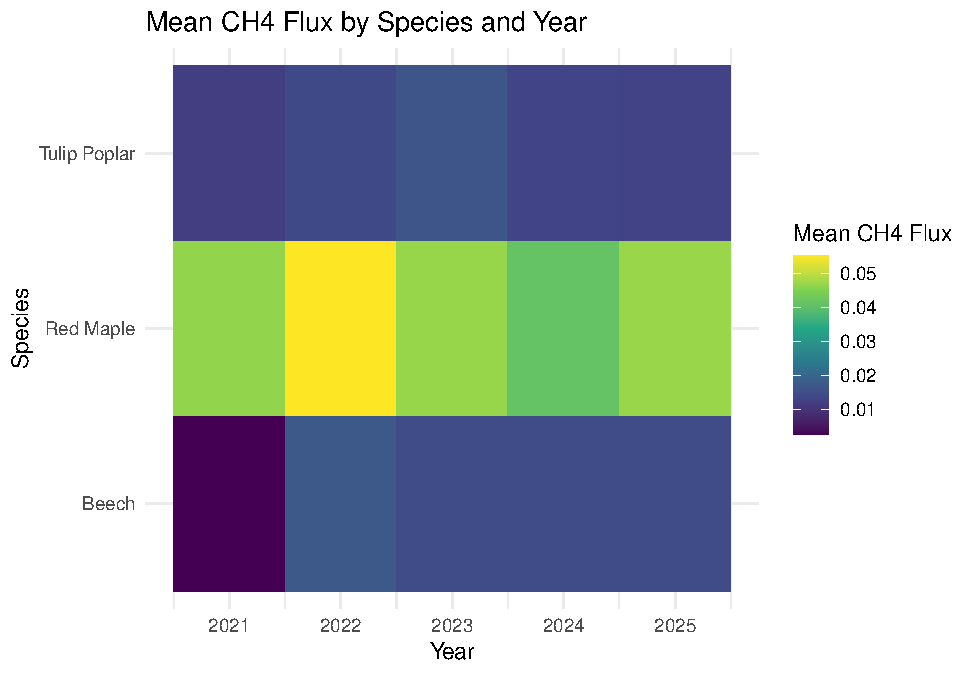
\includegraphics[keepaspectratio]{Mullen_TreeFlux_Analysis_files/Mullen_TreeFlux_Analysis_files/figure-latex/unnamed-chunk-8-1.pdf}}

\begin{Shaded}
\begin{Highlighting}[]
\NormalTok{seawater\_rows }\OtherTok{\textless{}{-}}\NormalTok{ my\_data }\SpecialCharTok{\%\textgreater{}\%}
  \FunctionTok{filter}\NormalTok{(Plot }\SpecialCharTok{==} \StringTok{"Seawater"}\NormalTok{)}

\NormalTok{heat\_data\_CO2 }\OtherTok{\textless{}{-}}\NormalTok{ my\_data }\SpecialCharTok{\%\textgreater{}\%}
  \FunctionTok{group\_by}\NormalTok{(Species, Year) }\SpecialCharTok{\%\textgreater{}\%}
  \FunctionTok{summarize}\NormalTok{(}\AttributeTok{mean\_flux =} \FunctionTok{mean}\NormalTok{(CO2\_lin\_flux.estimate, }\AttributeTok{na.rm =} \ConstantTok{TRUE}\NormalTok{),}\AttributeTok{.groups =} \StringTok{"drop"}\NormalTok{)}
\FunctionTok{ggplot}\NormalTok{(heat\_data\_CO2,}\FunctionTok{aes}\NormalTok{(}\AttributeTok{x =}\NormalTok{ Year, }\AttributeTok{y =}\NormalTok{ Species, }\AttributeTok{fill =}\NormalTok{ mean\_flux)) }\SpecialCharTok{+}
  \FunctionTok{geom\_tile}\NormalTok{() }\SpecialCharTok{+}
  \FunctionTok{scale\_fill\_viridis\_c}\NormalTok{() }\SpecialCharTok{+}
  \FunctionTok{labs}\NormalTok{(}\AttributeTok{title =} \StringTok{"Mean CO2 Flux by Species and Year"}\NormalTok{, }\AttributeTok{x =} \StringTok{"Year"}\NormalTok{,}\AttributeTok{y =} \StringTok{"Species"}\NormalTok{,}
       \AttributeTok{fill =} \StringTok{"Mean CO2 Flux"}\NormalTok{ ) }\SpecialCharTok{+}\FunctionTok{theme\_minimal}\NormalTok{()}
\end{Highlighting}
\end{Shaded}

\pandocbounded{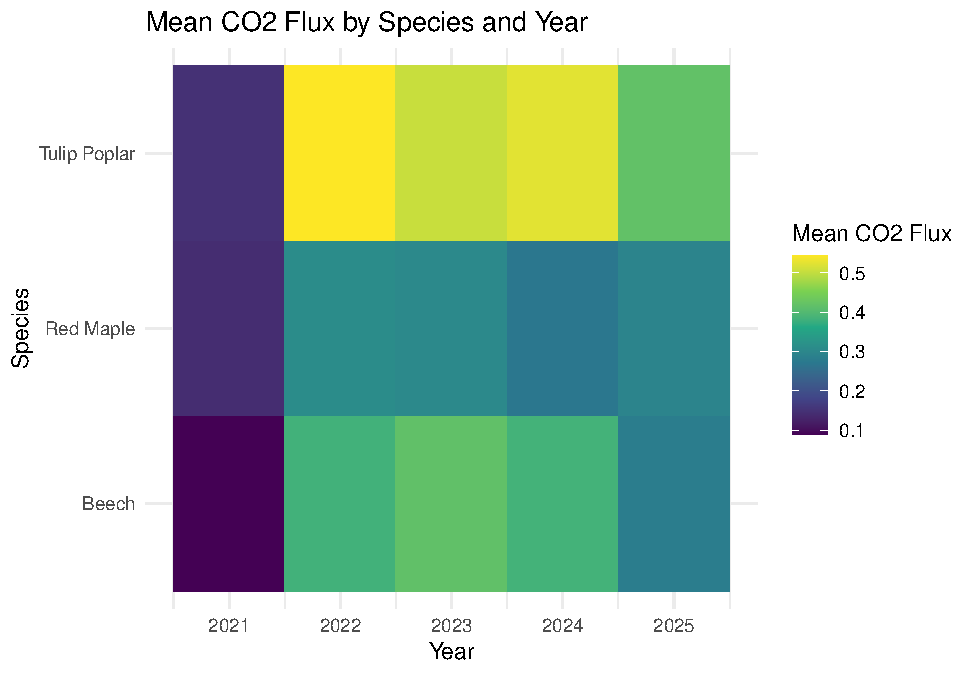
\includegraphics[keepaspectratio]{Mullen_TreeFlux_Analysis_files/Mullen_TreeFlux_Analysis_files/figure-latex/unnamed-chunk-8-2.pdf}}

\subsection{Relationship Between CH₄ and CO₂ Flux by
Species}\label{relationship-between-chux2084-and-coux2082-flux-by-species}

\begin{Shaded}
\begin{Highlighting}[]
\FunctionTok{ggplot}\NormalTok{(my\_data, }\FunctionTok{aes}\NormalTok{(}\AttributeTok{x =}\NormalTok{ CO2\_lin\_flux.estimate, }\AttributeTok{y =}\NormalTok{ CH4\_lin\_flux.estimate, }\AttributeTok{color =}\NormalTok{ Species)) }\SpecialCharTok{+}
  \FunctionTok{geom\_point}\NormalTok{(}\AttributeTok{alpha =} \FloatTok{0.4}\NormalTok{) }\SpecialCharTok{+}
  \FunctionTok{geom\_smooth}\NormalTok{(}\AttributeTok{method =} \StringTok{"lm"}\NormalTok{, }\AttributeTok{se =} \ConstantTok{FALSE}\NormalTok{) }\SpecialCharTok{+}
  \FunctionTok{labs}\NormalTok{(}\AttributeTok{title =} \StringTok{"Relationship Between CO2 and CH4 Flux by Species"}\NormalTok{,}\AttributeTok{x =} \StringTok{"CO2 Flux"}\NormalTok{,}\AttributeTok{y =} \StringTok{"CH4 Flux"}\NormalTok{,}
       \AttributeTok{color =} \StringTok{"Species"}\NormalTok{) }\SpecialCharTok{+}
  \FunctionTok{theme\_minimal}\NormalTok{()}
\end{Highlighting}
\end{Shaded}

\begin{verbatim}
## `geom_smooth()` using formula = 'y ~ x'
\end{verbatim}

\pandocbounded{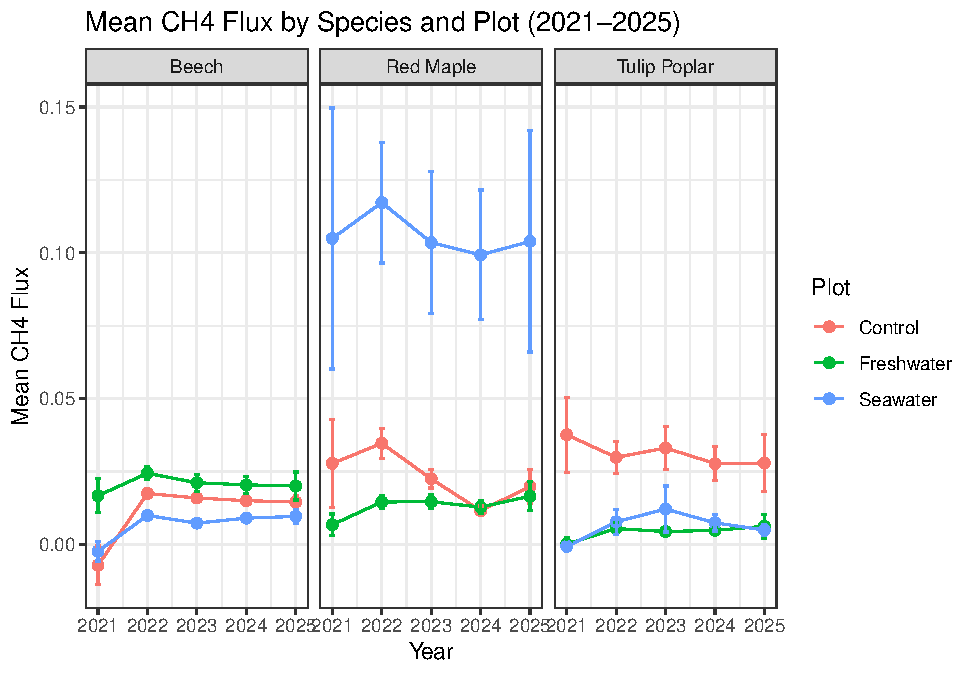
\includegraphics[keepaspectratio]{Mullen_TreeFlux_Analysis_files/Mullen_TreeFlux_Analysis_files/figure-latex/unnamed-chunk-9-1.pdf}}

\subsection{Quarterly Flux for both GHG (raw
data)}\label{quarterly-flux-for-both-ghg-raw-data}

\begin{Shaded}
\begin{Highlighting}[]
\NormalTok{annual\_means\_CH4 }\OtherTok{\textless{}{-}}\NormalTok{ my\_data }\SpecialCharTok{\%\textgreater{}\%}
  \FunctionTok{group\_by}\NormalTok{(Year, Species, Plot) }\SpecialCharTok{\%\textgreater{}\%}
  \FunctionTok{summarize}\NormalTok{( }\AttributeTok{mean\_flux =} \FunctionTok{mean}\NormalTok{(CH4\_lin\_flux.estimate, }\AttributeTok{na.rm =} \ConstantTok{TRUE}\NormalTok{),}
             \AttributeTok{se =} \FunctionTok{sd}\NormalTok{(CH4\_lin\_flux.estimate, }\AttributeTok{na.rm =} \ConstantTok{TRUE}\NormalTok{) }\SpecialCharTok{/} \FunctionTok{sqrt}\NormalTok{(}\FunctionTok{n}\NormalTok{()), }\AttributeTok{.groups =} \StringTok{"drop"}\NormalTok{)}
\FunctionTok{ggplot}\NormalTok{(annual\_means\_CH4, }\FunctionTok{aes}\NormalTok{( }\AttributeTok{x =}\NormalTok{ Year, }\AttributeTok{y =}\NormalTok{ mean\_flux,}\AttributeTok{color =}\NormalTok{ Plot,}\AttributeTok{group =}\NormalTok{ Plot)) }\SpecialCharTok{+}
  \FunctionTok{geom\_line}\NormalTok{() }\SpecialCharTok{+}
  \FunctionTok{geom\_point}\NormalTok{(}\AttributeTok{size =} \DecValTok{2}\NormalTok{) }\SpecialCharTok{+}
  \FunctionTok{geom\_errorbar}\NormalTok{( }\FunctionTok{aes}\NormalTok{(  }\AttributeTok{ymin =}\NormalTok{ mean\_flux }\SpecialCharTok{{-}}\NormalTok{ se,}\AttributeTok{ymax =}\NormalTok{ mean\_flux }\SpecialCharTok{+}\NormalTok{ se  ),}\AttributeTok{width =} \FloatTok{0.1}\NormalTok{ ) }\SpecialCharTok{+}
  \FunctionTok{facet\_wrap}\NormalTok{(}\SpecialCharTok{\textasciitilde{}}\NormalTok{ Species) }\SpecialCharTok{+}
  \FunctionTok{labs}\NormalTok{( }\AttributeTok{title =} \StringTok{"Mean CH4 Flux by Species and Plot (2021–2025)"}\NormalTok{,}
        \AttributeTok{x =} \StringTok{"Year"}\NormalTok{, }\AttributeTok{y =} \StringTok{"Mean CH4 Flux"}\NormalTok{ ) }
\end{Highlighting}
\end{Shaded}

\pandocbounded{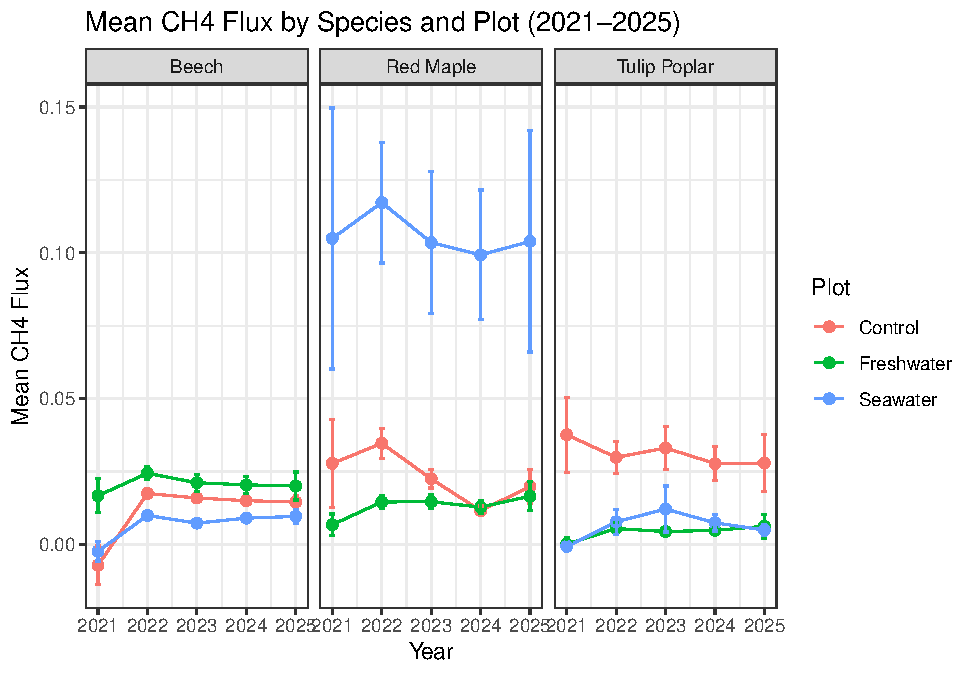
\includegraphics[keepaspectratio]{Mullen_TreeFlux_Analysis_files/Mullen_TreeFlux_Analysis_files/figure-latex/unnamed-chunk-10-1.pdf}}

\begin{Shaded}
\begin{Highlighting}[]
\NormalTok{annual\_means\_CO2 }\OtherTok{\textless{}{-}}\NormalTok{ my\_data }\SpecialCharTok{\%\textgreater{}\%}
  \FunctionTok{group\_by}\NormalTok{(Year, Species, Plot) }\SpecialCharTok{\%\textgreater{}\%}
  \FunctionTok{summarize}\NormalTok{( }\AttributeTok{mean\_flux =} \FunctionTok{mean}\NormalTok{(CO2\_lin\_flux.estimate, }\AttributeTok{na.rm =} \ConstantTok{TRUE}\NormalTok{),}
             \AttributeTok{se =} \FunctionTok{sd}\NormalTok{(CO2\_lin\_flux.estimate, }\AttributeTok{na.rm =} \ConstantTok{TRUE}\NormalTok{) }\SpecialCharTok{/} \FunctionTok{sqrt}\NormalTok{(}\FunctionTok{n}\NormalTok{()), }\AttributeTok{.groups =} \StringTok{"drop"}\NormalTok{)}
\FunctionTok{ggplot}\NormalTok{(annual\_means\_CO2,}\FunctionTok{aes}\NormalTok{( }\AttributeTok{x =}\NormalTok{ Year, }\AttributeTok{y =}\NormalTok{ mean\_flux, }\AttributeTok{color =}\NormalTok{ Plot, }\AttributeTok{group =}\NormalTok{ Plot  )) }\SpecialCharTok{+}
  \FunctionTok{geom\_line}\NormalTok{() }\SpecialCharTok{+}
  \FunctionTok{geom\_point}\NormalTok{(}\AttributeTok{size =} \DecValTok{2}\NormalTok{) }\SpecialCharTok{+}
  \FunctionTok{geom\_errorbar}\NormalTok{( }\FunctionTok{aes}\NormalTok{(}\AttributeTok{ymin =}\NormalTok{ mean\_flux }\SpecialCharTok{{-}}\NormalTok{ se,}\AttributeTok{ymax =}\NormalTok{ mean\_flux }\SpecialCharTok{+}\NormalTok{ se ), }\AttributeTok{width =} \FloatTok{0.1}\NormalTok{) }\SpecialCharTok{+}
  \FunctionTok{facet\_wrap}\NormalTok{(}\SpecialCharTok{\textasciitilde{}}\NormalTok{ Species) }\SpecialCharTok{+}
  \FunctionTok{labs}\NormalTok{( }\AttributeTok{title =} \StringTok{"Mean CO2 Flux by Species and Plot (2021–2025)"}\NormalTok{,}
        \AttributeTok{x =} \StringTok{"Year"}\NormalTok{,}
        \AttributeTok{y =} \StringTok{"Mean CO2 Flux"}\NormalTok{ ) }
\end{Highlighting}
\end{Shaded}

\pandocbounded{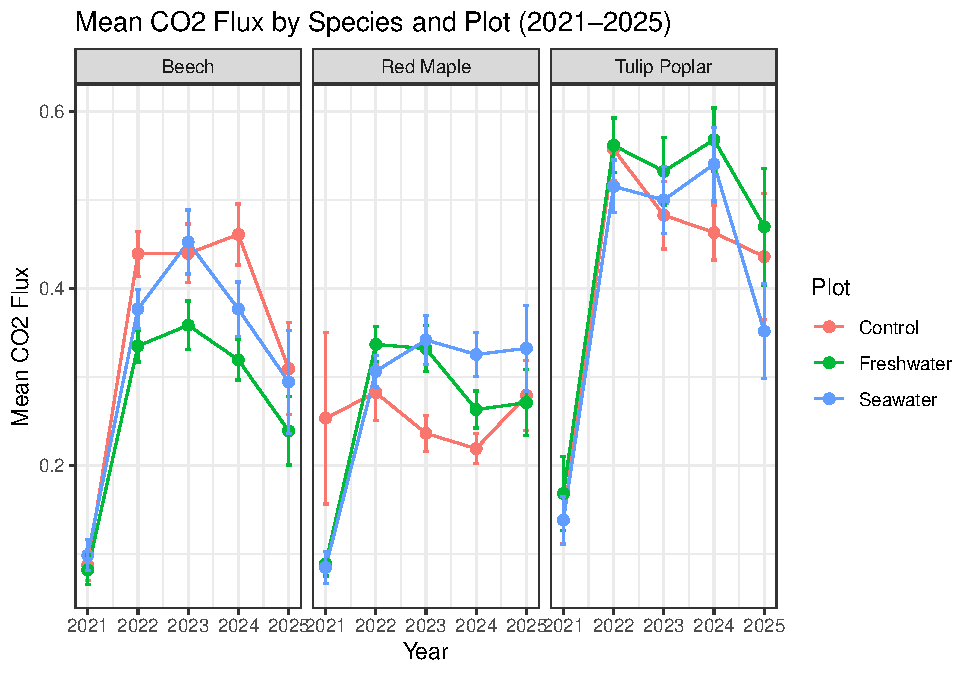
\includegraphics[keepaspectratio]{Mullen_TreeFlux_Analysis_files/Mullen_TreeFlux_Analysis_files/figure-latex/unnamed-chunk-10-2.pdf}}

\section{Creation of Quarters}\label{creation-of-quarters}

\begin{Shaded}
\begin{Highlighting}[]
\NormalTok{my\_data }\OtherTok{\textless{}{-}}\NormalTok{ my\_data }\SpecialCharTok{\%\textgreater{}\%}
  \FunctionTok{mutate}\NormalTok{(}
    \AttributeTok{Date =} \FunctionTok{as.Date}\NormalTok{(Date),}
    \AttributeTok{Year =} \FunctionTok{year}\NormalTok{(Date),}
    \AttributeTok{Quarter =} \FunctionTok{quarter}\NormalTok{(Date),}
    \AttributeTok{YearQuarter =}\NormalTok{ Year }\SpecialCharTok{+}\NormalTok{ (Quarter}\DecValTok{{-}1}\NormalTok{)}\SpecialCharTok{/}\DecValTok{4}\NormalTok{)}

\FunctionTok{table}\NormalTok{(my\_data}\SpecialCharTok{$}\NormalTok{Quarter)}
\end{Highlighting}
\end{Shaded}

\begin{verbatim}
## 
##    1    2    3    4 
##  539 1513  717  592
\end{verbatim}

\begin{Shaded}
\begin{Highlighting}[]
\NormalTok{quarterly\_CH4 }\OtherTok{\textless{}{-}}\NormalTok{ my\_data }\SpecialCharTok{\%\textgreater{}\%}
  \FunctionTok{mutate}\NormalTok{(}\AttributeTok{is\_S7 =}\NormalTok{ ID }\SpecialCharTok{==} \StringTok{"S7"}\NormalTok{) }\SpecialCharTok{\%\textgreater{}\%}
  \FunctionTok{group\_by}\NormalTok{(YearQuarter, Species, Plot, is\_S7) }\SpecialCharTok{\%\textgreater{}\%}
  \FunctionTok{summarize}\NormalTok{(}\AttributeTok{mean\_flux =} \FunctionTok{mean}\NormalTok{(CH4\_lin\_flux.estimate, }\AttributeTok{na.rm =} \ConstantTok{TRUE}\NormalTok{),}
            \AttributeTok{se =} \FunctionTok{sd}\NormalTok{(CH4\_lin\_flux.estimate, }\AttributeTok{na.rm =} \ConstantTok{TRUE}\NormalTok{) }\SpecialCharTok{/} \FunctionTok{sqrt}\NormalTok{(}\FunctionTok{n}\NormalTok{()), }\AttributeTok{.groups =} \StringTok{"drop"}\NormalTok{)}
\end{Highlighting}
\end{Shaded}

\section{Flood-week averages for
reference}\label{flood-week-averages-for-reference}

\begin{Shaded}
\begin{Highlighting}[]
\NormalTok{flood\_data }\OtherTok{\textless{}{-}} \FunctionTok{list}\NormalTok{()}
\ControlFlowTok{for}\NormalTok{(i }\ControlFlowTok{in} \FunctionTok{seq\_len}\NormalTok{(}\FunctionTok{nrow}\NormalTok{(flood\_date))) \{}
  \FunctionTok{message}\NormalTok{(}\StringTok{"Isolating data for "}\NormalTok{, flood\_date}\SpecialCharTok{$}\NormalTok{Event[i])}
\NormalTok{  flood\_data[[i]] }\OtherTok{\textless{}{-}}
\NormalTok{    my\_data }\SpecialCharTok{\%\textgreater{}\%}
    \FunctionTok{filter}\NormalTok{(}
\NormalTok{      Date }\SpecialCharTok{\textgreater{}=}\NormalTok{ flood\_date}\SpecialCharTok{$}\NormalTok{Start[i],}
\NormalTok{      Date }\SpecialCharTok{\textless{}=}\NormalTok{ flood\_date}\SpecialCharTok{$}\NormalTok{End[i]  ) }\SpecialCharTok{\%\textgreater{}\%}
    \FunctionTok{mutate}\NormalTok{(}\AttributeTok{Event =}\NormalTok{ flood\_date}\SpecialCharTok{$}\NormalTok{Event[i])\}}
\end{Highlighting}
\end{Shaded}

\begin{verbatim}
## Isolating data for T1
\end{verbatim}

\begin{verbatim}
## Isolating data for T2
\end{verbatim}

\begin{verbatim}
## Isolating data for T3
\end{verbatim}

\begin{Shaded}
\begin{Highlighting}[]
\NormalTok{flood\_CH4 }\OtherTok{\textless{}{-}} \FunctionTok{bind\_rows}\NormalTok{(flood\_data) }\SpecialCharTok{\%\textgreater{}\%}
  \FunctionTok{mutate}\NormalTok{(}\AttributeTok{is\_S7 =}\NormalTok{ ID }\SpecialCharTok{==} \StringTok{"S7"}\NormalTok{) }\SpecialCharTok{\%\textgreater{}\%}
  \FunctionTok{group\_by}\NormalTok{(Event, YearQuarter, Species, Plot, is\_S7) }\SpecialCharTok{\%\textgreater{}\%}
  \FunctionTok{summarize}\NormalTok{(}
    \AttributeTok{mean\_flux =} \FunctionTok{mean}\NormalTok{(CH4\_lin\_flux.estimate, }\AttributeTok{na.rm =} \ConstantTok{TRUE}\NormalTok{),}
    \AttributeTok{se =} \FunctionTok{sd}\NormalTok{(CH4\_lin\_flux.estimate, }\AttributeTok{na.rm =} \ConstantTok{TRUE}\NormalTok{) }\SpecialCharTok{/} \FunctionTok{sqrt}\NormalTok{(}\FunctionTok{n}\NormalTok{()),}
    \AttributeTok{.groups =} \StringTok{"drop"}\NormalTok{ )}
\end{Highlighting}
\end{Shaded}

\section{Quarterly Methane Flux with flood averages
emphasized}\label{quarterly-methane-flux-with-flood-averages-emphasized}

\begin{Shaded}
\begin{Highlighting}[]
\FunctionTok{ggplot}\NormalTok{(quarterly\_CH4,}
       \FunctionTok{aes}\NormalTok{(}\AttributeTok{x =}\NormalTok{ YearQuarter, }\AttributeTok{y =}\NormalTok{ mean\_flux, }\AttributeTok{color =}\NormalTok{ Plot, }\AttributeTok{group =}\NormalTok{ Plot)) }\SpecialCharTok{+}
  \FunctionTok{geom\_line}\NormalTok{() }\SpecialCharTok{+}
  \FunctionTok{geom\_point}\NormalTok{(}\AttributeTok{size =} \DecValTok{2}\NormalTok{) }\SpecialCharTok{+}
  \FunctionTok{geom\_errorbar}\NormalTok{(}
    \FunctionTok{aes}\NormalTok{(}\AttributeTok{ymin =}\NormalTok{ mean\_flux }\SpecialCharTok{{-}}\NormalTok{ se,}
        \AttributeTok{ymax =}\NormalTok{ mean\_flux }\SpecialCharTok{+}\NormalTok{ se),}
    \AttributeTok{width =} \FloatTok{0.05}\NormalTok{) }\SpecialCharTok{+}
  \CommentTok{\# Flood overlay (T1, T2, T3 labeled in legend)}
  \FunctionTok{geom\_point}\NormalTok{(}
    \AttributeTok{data =}\NormalTok{ flood\_CH4,}
    \FunctionTok{aes}\NormalTok{(}\AttributeTok{x =}\NormalTok{ YearQuarter,}
        \AttributeTok{y =}\NormalTok{ mean\_flux,}
        \AttributeTok{shape =}\NormalTok{ Event),}
    \AttributeTok{color =} \StringTok{"black"}\NormalTok{,}
    \AttributeTok{size =} \FloatTok{1.5}\NormalTok{,}
    \AttributeTok{inherit.aes =} \ConstantTok{FALSE}\NormalTok{) }\SpecialCharTok{+}
  \FunctionTok{facet\_wrap}\NormalTok{(}\SpecialCharTok{\textasciitilde{}}\NormalTok{ Species) }\SpecialCharTok{+}
  \FunctionTok{labs}\NormalTok{( }\AttributeTok{title =} \StringTok{"Quarterly CH4 Flux with Flood Events Highlighted"}\NormalTok{,}
        \AttributeTok{x =} \StringTok{"Year{-}Quarter"}\NormalTok{,}
        \AttributeTok{y =} \StringTok{"CH4 Flux"}\NormalTok{,}
        \AttributeTok{shape =} \StringTok{"Flood event"}\NormalTok{) }\SpecialCharTok{+}
  \FunctionTok{scale\_shape\_manual}\NormalTok{(}\AttributeTok{values =} \FunctionTok{c}\NormalTok{(}
    \AttributeTok{T1 =} \DecValTok{17}\NormalTok{,}
    \AttributeTok{T2 =} \DecValTok{17}\NormalTok{,}
    \AttributeTok{T3 =} \DecValTok{17}\NormalTok{)) }\SpecialCharTok{+}
  \FunctionTok{theme}\NormalTok{(}\AttributeTok{axis.text.x =} \FunctionTok{element\_text}\NormalTok{(}\AttributeTok{angle =} \DecValTok{45}\NormalTok{, }\AttributeTok{hjust =} \DecValTok{1}\NormalTok{))}
\end{Highlighting}
\end{Shaded}

\pandocbounded{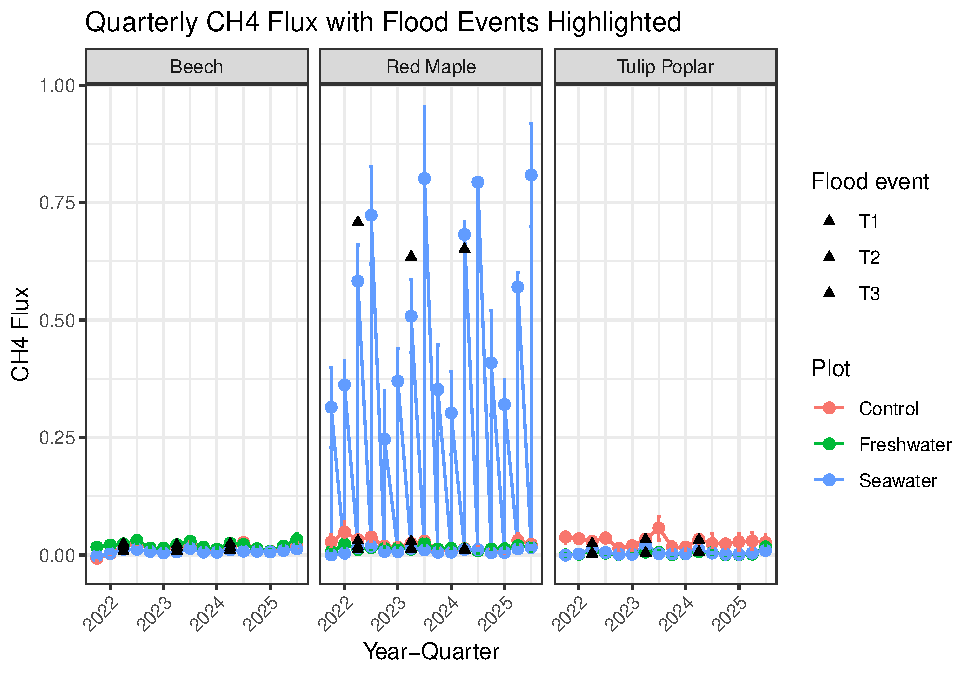
\includegraphics[keepaspectratio]{Mullen_TreeFlux_Analysis_files/Mullen_TreeFlux_Analysis_files/figure-latex/unnamed-chunk-14-1.pdf}}

\section{Isolating Red Maple Trees (finding outlier
(S7))}\label{isolating-red-maple-trees-finding-outlier-s7}

\begin{Shaded}
\begin{Highlighting}[]
\NormalTok{my\_data }\SpecialCharTok{\%\textgreater{}\%}
  \FunctionTok{filter}\NormalTok{(Species }\SpecialCharTok{==} \StringTok{"Red Maple"}\NormalTok{) }\SpecialCharTok{\%\textgreater{}\%}
  \FunctionTok{ggplot}\NormalTok{(}\FunctionTok{aes}\NormalTok{(}\AttributeTok{x =}\NormalTok{ Date, }\AttributeTok{y =}\NormalTok{ CH4\_lin\_flux.estimate)) }\SpecialCharTok{+}
  \FunctionTok{geom\_line}\NormalTok{(}\AttributeTok{alpha =} \FloatTok{0.7}\NormalTok{) }\SpecialCharTok{+}
  \FunctionTok{facet\_wrap}\NormalTok{(}\SpecialCharTok{\textasciitilde{}}\NormalTok{ ID) }\SpecialCharTok{+}
  \FunctionTok{labs}\NormalTok{(}\AttributeTok{title =} \StringTok{"Red Maple CH4 Flux by Individual Tree"}\NormalTok{)}
\end{Highlighting}
\end{Shaded}

\pandocbounded{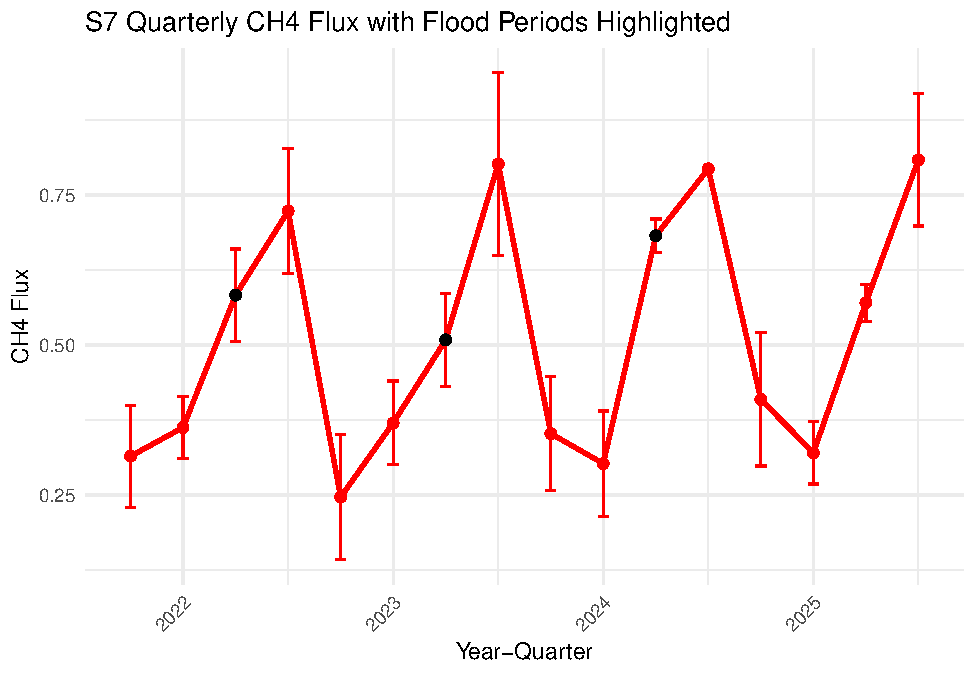
\includegraphics[keepaspectratio]{Mullen_TreeFlux_Analysis_files/Mullen_TreeFlux_Analysis_files/figure-latex/unnamed-chunk-15-1.pdf}}

\begin{Shaded}
\begin{Highlighting}[]
\NormalTok{my\_data }\SpecialCharTok{\%\textgreater{}\%}
  \FunctionTok{filter}\NormalTok{(Species }\SpecialCharTok{==} \StringTok{"Red Maple"}\NormalTok{) }\SpecialCharTok{\%\textgreater{}\%}
  \FunctionTok{ggplot}\NormalTok{(}\FunctionTok{aes}\NormalTok{(}\AttributeTok{x =}\NormalTok{ Date, }\AttributeTok{y =}\NormalTok{ CO2\_lin\_flux.estimate)) }\SpecialCharTok{+}
  \FunctionTok{geom\_line}\NormalTok{(}\AttributeTok{alpha =} \FloatTok{0.7}\NormalTok{) }\SpecialCharTok{+}
  \FunctionTok{facet\_wrap}\NormalTok{(}\SpecialCharTok{\textasciitilde{}}\NormalTok{ ID) }
\end{Highlighting}
\end{Shaded}

\pandocbounded{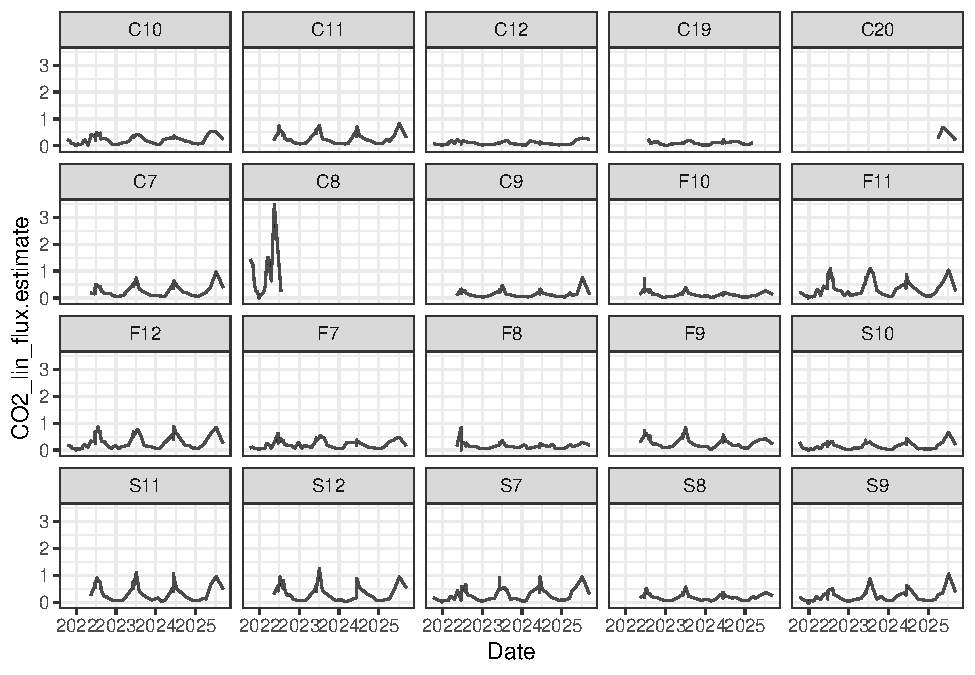
\includegraphics[keepaspectratio]{Mullen_TreeFlux_Analysis_files/Mullen_TreeFlux_Analysis_files/figure-latex/unnamed-chunk-15-2.pdf}}

\section{Separate S7 from all other
trees}\label{separate-s7-from-all-other-trees}

\begin{Shaded}
\begin{Highlighting}[]
\NormalTok{s7\_CH4 }\OtherTok{\textless{}{-}}\NormalTok{ my\_data }\SpecialCharTok{\%\textgreater{}\%}
  \FunctionTok{filter}\NormalTok{(ID }\SpecialCharTok{==} \StringTok{"S7"}\NormalTok{) }\SpecialCharTok{\%\textgreater{}\%}
  \FunctionTok{group\_by}\NormalTok{(YearQuarter, Species, Plot) }\SpecialCharTok{\%\textgreater{}\%}
  \FunctionTok{summarize}\NormalTok{(}\AttributeTok{mean\_flux =} \FunctionTok{mean}\NormalTok{(CH4\_lin\_flux.estimate, }\AttributeTok{na.rm =} \ConstantTok{TRUE}\NormalTok{),}
            \AttributeTok{se =} \FunctionTok{sd}\NormalTok{(CH4\_lin\_flux.estimate, }\AttributeTok{na.rm =} \ConstantTok{TRUE}\NormalTok{) }\SpecialCharTok{/} \FunctionTok{sqrt}\NormalTok{(}\FunctionTok{n}\NormalTok{()), }\AttributeTok{.groups =} \StringTok{"drop"}\NormalTok{  )}
\NormalTok{quarterly\_CH4\_nos7 }\OtherTok{\textless{}{-}}\NormalTok{ my\_data }\SpecialCharTok{\%\textgreater{}\%}
  \FunctionTok{filter}\NormalTok{(ID }\SpecialCharTok{!=} \StringTok{"S7"}\NormalTok{) }\SpecialCharTok{\%\textgreater{}\%}
  \FunctionTok{group\_by}\NormalTok{(YearQuarter, Species, Plot) }\SpecialCharTok{\%\textgreater{}\%}
  \FunctionTok{summarize}\NormalTok{(}\AttributeTok{mean\_flux =} \FunctionTok{mean}\NormalTok{(CH4\_lin\_flux.estimate, }\AttributeTok{na.rm =} \ConstantTok{TRUE}\NormalTok{),}
            \AttributeTok{se =} \FunctionTok{sd}\NormalTok{(CH4\_lin\_flux.estimate, }\AttributeTok{na.rm =} \ConstantTok{TRUE}\NormalTok{) }\SpecialCharTok{/} \FunctionTok{sqrt}\NormalTok{(}\FunctionTok{n}\NormalTok{()), }\AttributeTok{.groups =} \StringTok{"drop"}\NormalTok{ )}
\NormalTok{quarterly\_CH4\_S7 }\OtherTok{\textless{}{-}}\NormalTok{ s7\_CH4}
\NormalTok{flood\_points }\OtherTok{\textless{}{-}}\NormalTok{ flood\_date }\SpecialCharTok{\%\textgreater{}\%}
  \FunctionTok{mutate}\NormalTok{(}\AttributeTok{YearQuarter =} \FunctionTok{year}\NormalTok{(Start) }\SpecialCharTok{+}\NormalTok{ (}\FunctionTok{quarter}\NormalTok{(Start)}\SpecialCharTok{{-}}\DecValTok{1}\NormalTok{)}\SpecialCharTok{/}\DecValTok{4}\NormalTok{) }\SpecialCharTok{\%\textgreater{}\%}
  \FunctionTok{select}\NormalTok{(Event, YearQuarter)}
\NormalTok{flood\_S7\_CH4 }\OtherTok{\textless{}{-}}\NormalTok{ s7\_CH4 }\SpecialCharTok{\%\textgreater{}\%}
  \FunctionTok{inner\_join}\NormalTok{(flood\_points, }\AttributeTok{by =} \StringTok{"YearQuarter"}\NormalTok{)}
\end{Highlighting}
\end{Shaded}

\#Quarterly CH4 Flux (S7 excluded from means, shown separately)

\begin{Shaded}
\begin{Highlighting}[]
\FunctionTok{ggplot}\NormalTok{() }\SpecialCharTok{+}
  \CommentTok{\# OTHER TREES (baseline)}
  \FunctionTok{geom\_line}\NormalTok{(}
    \AttributeTok{data =}\NormalTok{ quarterly\_CH4\_nos7,}
    \FunctionTok{aes}\NormalTok{(}\AttributeTok{x =}\NormalTok{ YearQuarter, }\AttributeTok{y =}\NormalTok{ mean\_flux, }\AttributeTok{color =}\NormalTok{ Plot, }\AttributeTok{group =}\NormalTok{ Plot)) }\SpecialCharTok{+}
  \FunctionTok{geom\_point}\NormalTok{(}
    \AttributeTok{data =}\NormalTok{ quarterly\_CH4\_nos7,}
    \FunctionTok{aes}\NormalTok{(}\AttributeTok{x =}\NormalTok{ YearQuarter, }\AttributeTok{y =}\NormalTok{ mean\_flux, }\AttributeTok{color =}\NormalTok{ Plot)) }\SpecialCharTok{+}
  \CommentTok{\# S7 (highlighted)}
  \FunctionTok{geom\_line}\NormalTok{(}
    \AttributeTok{data =}\NormalTok{ s7\_CH4,}
    \FunctionTok{aes}\NormalTok{(}\AttributeTok{x =}\NormalTok{ YearQuarter, }\AttributeTok{y =}\NormalTok{ mean\_flux),}
    \AttributeTok{color =} \StringTok{"red"}\NormalTok{,}
    \AttributeTok{linewidth =} \DecValTok{1}\NormalTok{ ) }\SpecialCharTok{+}
  \FunctionTok{geom\_point}\NormalTok{(}\AttributeTok{data =}\NormalTok{ s7\_CH4,}
             \FunctionTok{aes}\NormalTok{(}\AttributeTok{x =}\NormalTok{ YearQuarter, }\AttributeTok{y =}\NormalTok{ mean\_flux),}
             \AttributeTok{color =} \StringTok{"red"}\NormalTok{, }\AttributeTok{size =} \DecValTok{2}\NormalTok{) }\SpecialCharTok{+}
  \CommentTok{\# FLOOD EVENTS ON S7 }
  \FunctionTok{geom\_point}\NormalTok{(}
    \AttributeTok{data =}\NormalTok{ s7\_CH4 }\SpecialCharTok{\%\textgreater{}\%}
      \FunctionTok{inner\_join}\NormalTok{(flood\_points, }\AttributeTok{by =} \StringTok{"YearQuarter"}\NormalTok{),}
    \FunctionTok{aes}\NormalTok{(}\AttributeTok{x =}\NormalTok{ YearQuarter, }\AttributeTok{y =}\NormalTok{ mean\_flux, }\AttributeTok{shape =}\NormalTok{ Event),}
    \AttributeTok{color =} \StringTok{"black"}\NormalTok{,}
    \AttributeTok{size =} \DecValTok{3}\NormalTok{ ) }\SpecialCharTok{+}
  \FunctionTok{facet\_wrap}\NormalTok{(}\SpecialCharTok{\textasciitilde{}}\NormalTok{ Species) }\SpecialCharTok{+}
  \FunctionTok{labs}\NormalTok{( }\AttributeTok{title =} \StringTok{"Quarterly CH4 Flux (S7 excluded from means, shown separately)"}\NormalTok{,}
        \AttributeTok{x =} \StringTok{"Year{-}Quarter"}\NormalTok{,}
        \AttributeTok{y =} \StringTok{"CH4 Flux"}\NormalTok{,}
        \AttributeTok{shape =} \StringTok{"Flood event"}\NormalTok{) }\SpecialCharTok{+}
  \FunctionTok{scale\_shape\_manual}\NormalTok{(}\AttributeTok{values =} \FunctionTok{c}\NormalTok{(}
    \AttributeTok{T1 =} \DecValTok{17}\NormalTok{,}
    \AttributeTok{T2 =} \DecValTok{17}\NormalTok{,}
    \AttributeTok{T3 =} \DecValTok{17}\NormalTok{ )) }\SpecialCharTok{+}
  \FunctionTok{theme\_minimal}\NormalTok{() }\SpecialCharTok{+}
  \FunctionTok{theme}\NormalTok{(}\AttributeTok{axis.text.x =} \FunctionTok{element\_text}\NormalTok{(}\AttributeTok{angle =} \DecValTok{45}\NormalTok{, }\AttributeTok{hjust =} \DecValTok{1}\NormalTok{))}
\end{Highlighting}
\end{Shaded}

\pandocbounded{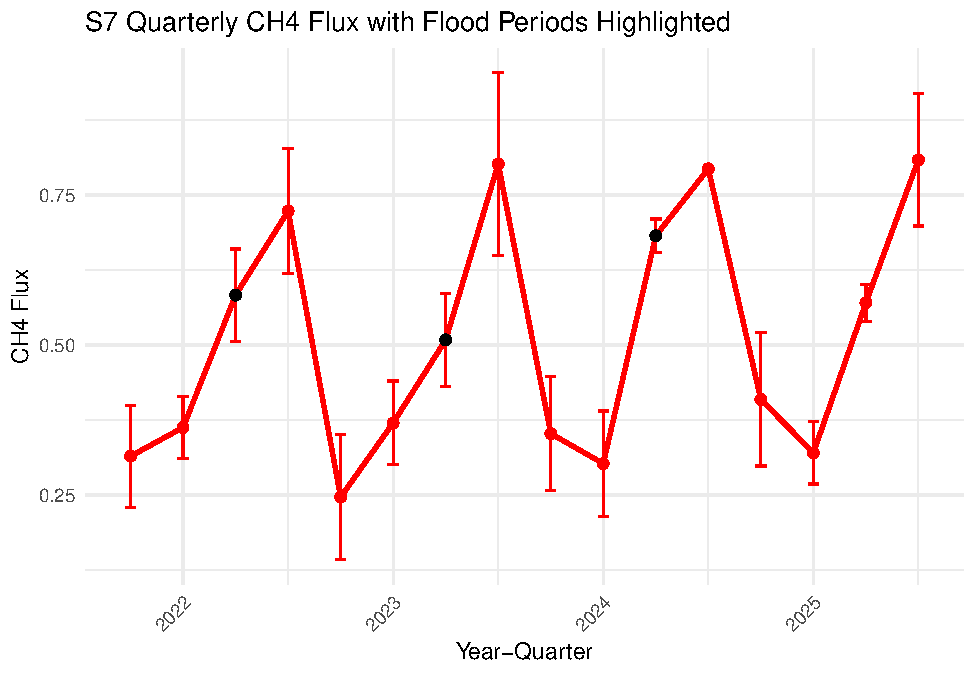
\includegraphics[keepaspectratio]{Mullen_TreeFlux_Analysis_files/Mullen_TreeFlux_Analysis_files/figure-latex/unnamed-chunk-17-1.pdf}}

\#S7 only

\begin{Shaded}
\begin{Highlighting}[]
\FunctionTok{ggplot}\NormalTok{(quarterly\_CH4\_S7, }\FunctionTok{aes}\NormalTok{(}\AttributeTok{x =}\NormalTok{ YearQuarter, }\AttributeTok{y =}\NormalTok{ mean\_flux)) }\SpecialCharTok{+}
  \FunctionTok{geom\_line}\NormalTok{(}\AttributeTok{color =} \StringTok{"red"}\NormalTok{, }\AttributeTok{linewidth =} \DecValTok{1}\NormalTok{) }\SpecialCharTok{+} \FunctionTok{geom\_point}\NormalTok{(}\AttributeTok{color =} \StringTok{"red"}\NormalTok{, }\AttributeTok{size =} \DecValTok{2}\NormalTok{) }\SpecialCharTok{+}
  \FunctionTok{geom\_errorbar}\NormalTok{(}\FunctionTok{aes}\NormalTok{(}\AttributeTok{ymin =}\NormalTok{ mean\_flux }\SpecialCharTok{{-}}\NormalTok{ se, }\AttributeTok{ymax =}\NormalTok{ mean\_flux }\SpecialCharTok{+}\NormalTok{ se),}
                \AttributeTok{width =} \FloatTok{0.05}\NormalTok{, }\AttributeTok{color =} \StringTok{"red"}\NormalTok{ ) }\SpecialCharTok{+}
  \FunctionTok{geom\_point}\NormalTok{(}
    \AttributeTok{data =}\NormalTok{ flood\_S7\_CH4,}
    \FunctionTok{aes}\NormalTok{(}\AttributeTok{x =}\NormalTok{ YearQuarter, }\AttributeTok{y =}\NormalTok{ mean\_flux),}
    \AttributeTok{color =} \StringTok{"black"}\NormalTok{,}
    \AttributeTok{size =} \DecValTok{2}\NormalTok{  ) }\SpecialCharTok{+}
  \FunctionTok{labs}\NormalTok{( }\AttributeTok{title =} \StringTok{"S7 Quarterly CH4 Flux with Flood Periods Highlighted"}\NormalTok{,}
        \AttributeTok{x =} \StringTok{"Year{-}Quarter"}\NormalTok{,}
        \AttributeTok{y =} \StringTok{"CH4 Flux"}\NormalTok{) }\SpecialCharTok{+}
  \FunctionTok{theme\_minimal}\NormalTok{() }\SpecialCharTok{+}
  \FunctionTok{theme}\NormalTok{(}\AttributeTok{axis.text.x =} \FunctionTok{element\_text}\NormalTok{(}\AttributeTok{angle =} \DecValTok{45}\NormalTok{, }\AttributeTok{hjust =} \DecValTok{1}\NormalTok{))}
\end{Highlighting}
\end{Shaded}

\pandocbounded{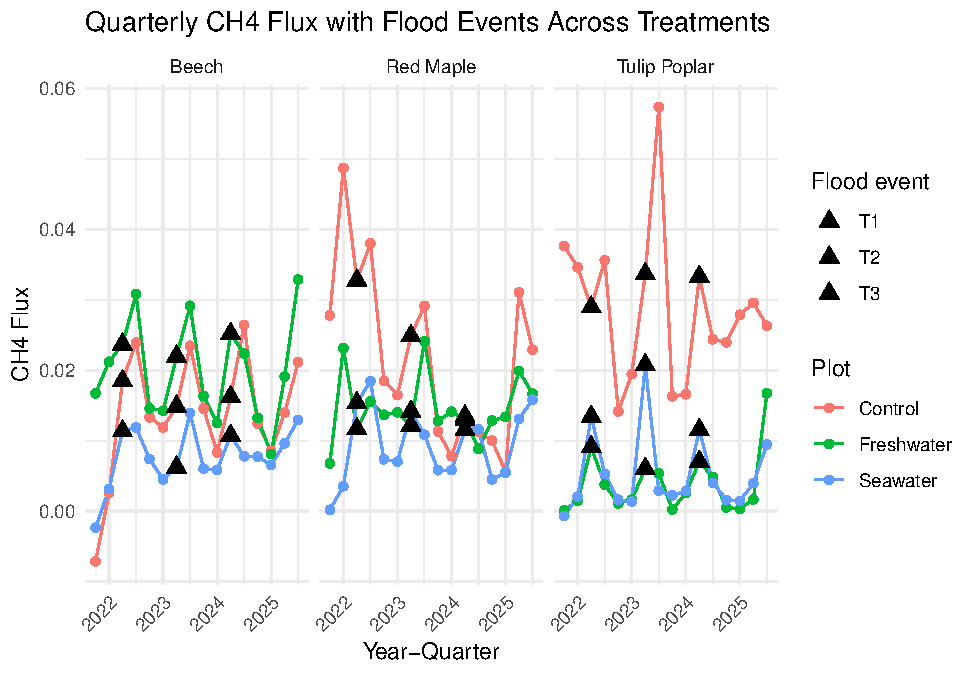
\includegraphics[keepaspectratio]{Mullen_TreeFlux_Analysis_files/Mullen_TreeFlux_Analysis_files/figure-latex/unnamed-chunk-18-1.pdf}}

\#S7 Excluded from CH4 Flux

\begin{Shaded}
\begin{Highlighting}[]
\NormalTok{flood\_plot\_data }\OtherTok{\textless{}{-}}\NormalTok{ quarterly\_CH4\_nos7 }\SpecialCharTok{\%\textgreater{}\%}
  \FunctionTok{inner\_join}\NormalTok{(flood\_points, }\AttributeTok{by =} \StringTok{"YearQuarter"}\NormalTok{)}
\FunctionTok{ggplot}\NormalTok{() }\SpecialCharTok{+}  \FunctionTok{geom\_line}\NormalTok{(}
  \AttributeTok{data =}\NormalTok{ quarterly\_CH4\_nos7,}
  \FunctionTok{aes}\NormalTok{(}\AttributeTok{x =}\NormalTok{ YearQuarter, }\AttributeTok{y =}\NormalTok{ mean\_flux, }\AttributeTok{color =}\NormalTok{ Plot, }\AttributeTok{group =}\NormalTok{ Plot) ) }\SpecialCharTok{+}
  \FunctionTok{geom\_point}\NormalTok{(}
    \AttributeTok{data =}\NormalTok{ quarterly\_CH4\_nos7,}\FunctionTok{aes}\NormalTok{(}\AttributeTok{x =}\NormalTok{ YearQuarter, }\AttributeTok{y =}\NormalTok{ mean\_flux, }\AttributeTok{color =}\NormalTok{ Plot) ) }\SpecialCharTok{+}
  \FunctionTok{geom\_point}\NormalTok{(}\AttributeTok{data =}\NormalTok{ flood\_plot\_data,}
             \FunctionTok{aes}\NormalTok{(}\AttributeTok{x =}\NormalTok{ YearQuarter, }\AttributeTok{y =}\NormalTok{ mean\_flux, }\AttributeTok{shape =}\NormalTok{ Event),}
             \AttributeTok{color =} \StringTok{"black"}\NormalTok{,}
             \AttributeTok{size =} \DecValTok{3}\NormalTok{ ) }\SpecialCharTok{+}
  \FunctionTok{facet\_wrap}\NormalTok{(}\SpecialCharTok{\textasciitilde{}}\NormalTok{ Species) }\SpecialCharTok{+}
  \FunctionTok{labs}\NormalTok{(}\AttributeTok{title =} \StringTok{"Quarterly CH4 Flux with Flood Events Across Treatments"}\NormalTok{,}
       \AttributeTok{x =} \StringTok{"Year{-}Quarter"}\NormalTok{,}
       \AttributeTok{y =} \StringTok{"CH4 Flux"}\NormalTok{,}
       \AttributeTok{shape =} \StringTok{"Flood event"}\NormalTok{ ) }\SpecialCharTok{+}
  \FunctionTok{scale\_shape\_manual}\NormalTok{(}\AttributeTok{values =} \FunctionTok{c}\NormalTok{(}\AttributeTok{T1 =} \DecValTok{17}\NormalTok{, }\AttributeTok{T2 =} \DecValTok{17}\NormalTok{, }\AttributeTok{T3 =} \DecValTok{17}\NormalTok{)) }\SpecialCharTok{+}
  \FunctionTok{theme\_minimal}\NormalTok{() }\SpecialCharTok{+} \FunctionTok{theme}\NormalTok{(}\AttributeTok{axis.text.x =} \FunctionTok{element\_text}\NormalTok{(}\AttributeTok{angle =} \DecValTok{45}\NormalTok{, }\AttributeTok{hjust =} \DecValTok{1}\NormalTok{))}
\end{Highlighting}
\end{Shaded}

\pandocbounded{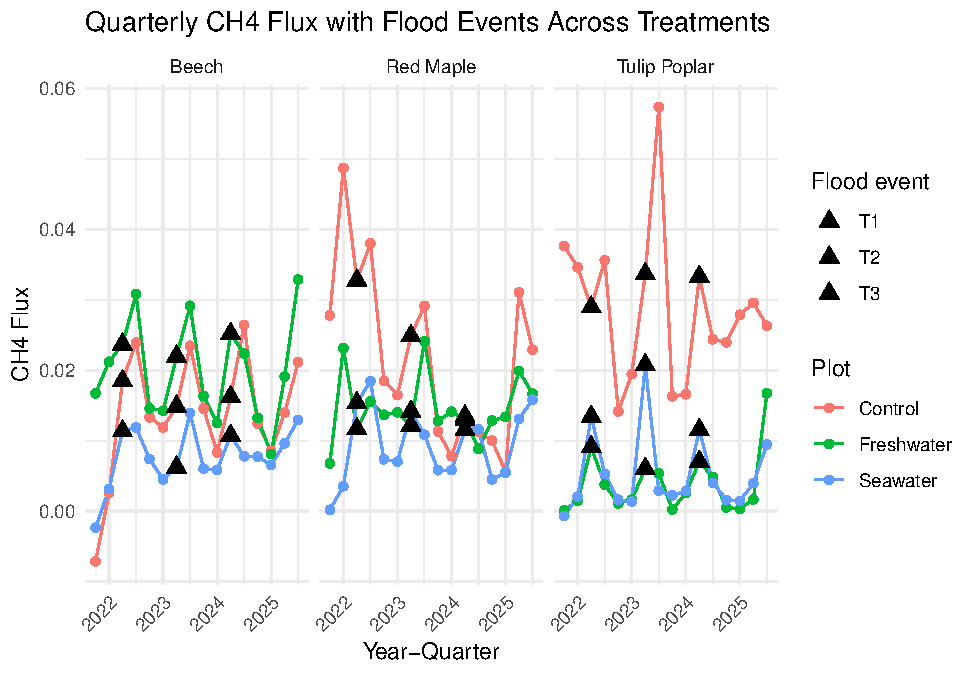
\includegraphics[keepaspectratio]{Mullen_TreeFlux_Analysis_files/Mullen_TreeFlux_Analysis_files/figure-latex/unnamed-chunk-19-1.pdf}}

\section{Visualizing Soil Temp Data x GHG Tree
Flux}\label{visualizing-soil-temp-data-x-ghg-tree-flux}

\subsection{GHG Tree Flux x Soil Temp (colored by
species)}\label{ghg-tree-flux-x-soil-temp-colored-by-species}

\begin{Shaded}
\begin{Highlighting}[]
\FunctionTok{ggplot}\NormalTok{(my\_data, }\FunctionTok{aes}\NormalTok{(}\AttributeTok{x =}\NormalTok{ soil\_temp\_daily\_mean,}
             \AttributeTok{y =}\NormalTok{ CH4\_lin\_flux.estimate,}
             \AttributeTok{color =}\NormalTok{ Species)) }\SpecialCharTok{+}
 \FunctionTok{geom\_point}\NormalTok{(}\AttributeTok{alpha =} \FloatTok{0.5}\NormalTok{) }\SpecialCharTok{+}
 \FunctionTok{geom\_smooth}\NormalTok{(}\AttributeTok{method =} \StringTok{"lm"}\NormalTok{, }\AttributeTok{se =} \ConstantTok{FALSE}\NormalTok{) }\SpecialCharTok{+}
 \FunctionTok{labs}\NormalTok{(}
     \AttributeTok{x =} \StringTok{"Daily Mean Soil Temperature (°C)"}\NormalTok{,}
     \AttributeTok{y =} \StringTok{"CH₄ Flux"}\NormalTok{ )}
\end{Highlighting}
\end{Shaded}

\begin{verbatim}
## `geom_smooth()` using formula = 'y ~ x'
\end{verbatim}

\pandocbounded{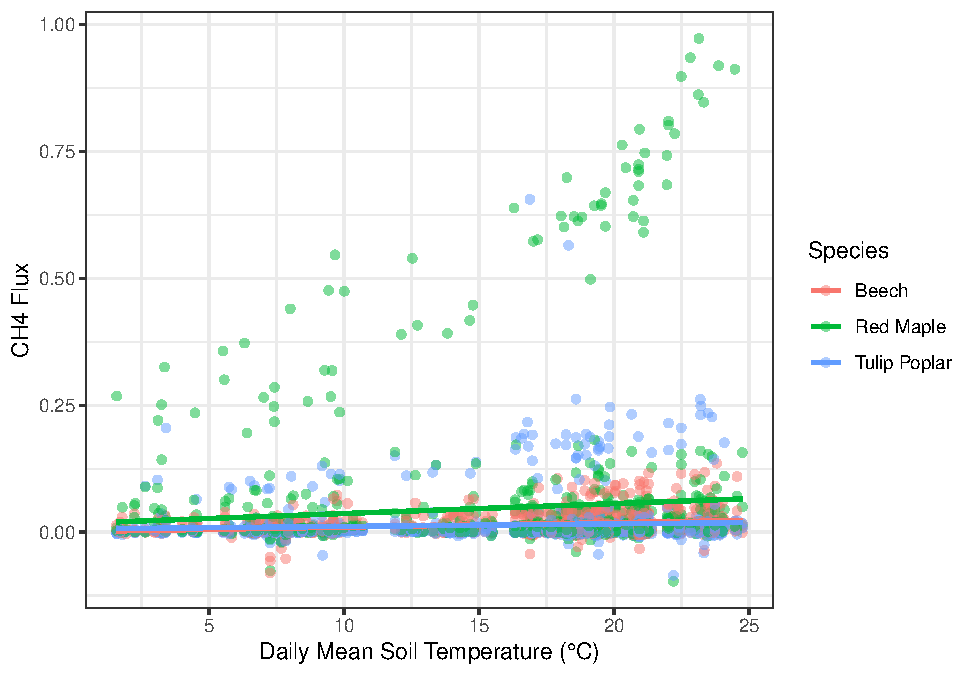
\includegraphics[keepaspectratio]{Mullen_TreeFlux_Analysis_files/Mullen_TreeFlux_Analysis_files/figure-latex/unnamed-chunk-20-1.pdf}}

\begin{Shaded}
\begin{Highlighting}[]
\FunctionTok{ggplot}\NormalTok{(my\_data,}\FunctionTok{aes}\NormalTok{(}\AttributeTok{x =}\NormalTok{ soil\_temp\_daily\_mean,}
                   \AttributeTok{y =}\NormalTok{ CO2\_lin\_flux.estimate,}
                   \AttributeTok{color =}\NormalTok{ Species)) }\SpecialCharTok{+}
\FunctionTok{geom\_point}\NormalTok{(}\AttributeTok{alpha =} \FloatTok{0.5}\NormalTok{) }\SpecialCharTok{+} \FunctionTok{geom\_smooth}\NormalTok{(}\AttributeTok{method =} \StringTok{"lm"}\NormalTok{, }\AttributeTok{se =} \ConstantTok{FALSE}\NormalTok{)}
\end{Highlighting}
\end{Shaded}

\begin{verbatim}
## `geom_smooth()` using formula = 'y ~ x'
\end{verbatim}

\pandocbounded{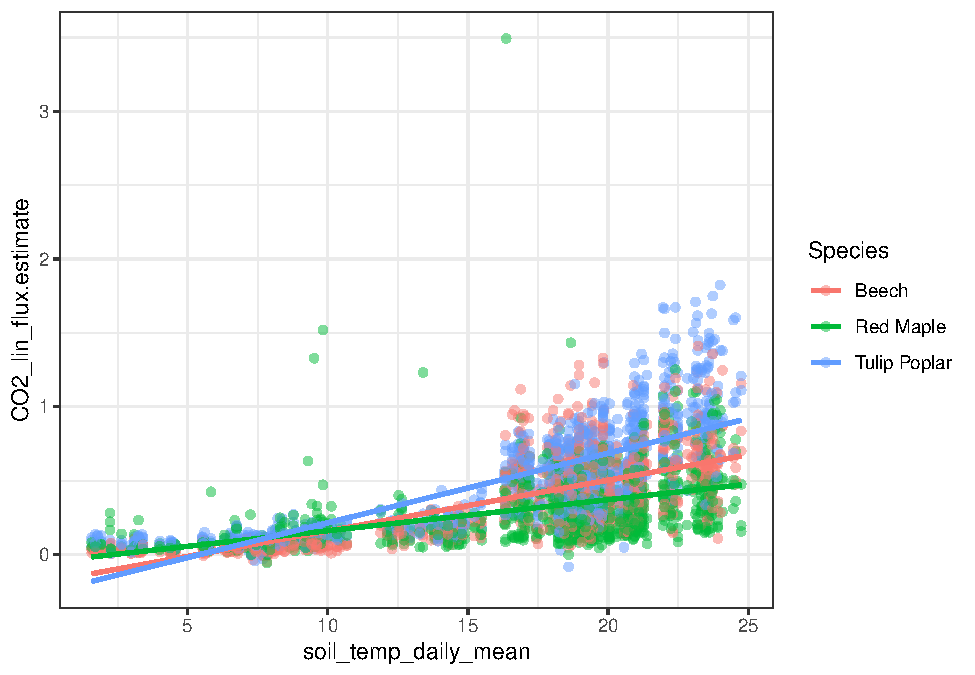
\includegraphics[keepaspectratio]{Mullen_TreeFlux_Analysis_files/Mullen_TreeFlux_Analysis_files/figure-latex/unnamed-chunk-20-2.pdf}}

\subsection{CH4 Tree Flux x Soil Temp (colored by
species)}\label{ch4-tree-flux-x-soil-temp-colored-by-species}

\begin{Shaded}
\begin{Highlighting}[]
\FunctionTok{ggplot}\NormalTok{(my\_data, }\FunctionTok{aes}\NormalTok{(}\AttributeTok{x =}\NormalTok{ soil\_temp\_daily\_mean,}
             \AttributeTok{y =}\NormalTok{ CH4\_lin\_flux.estimate,}
             \AttributeTok{color =}\NormalTok{ Species)) }\SpecialCharTok{+}
 \FunctionTok{geom\_point}\NormalTok{(}\AttributeTok{alpha =} \FloatTok{0.5}\NormalTok{) }\SpecialCharTok{+}
 \FunctionTok{geom\_smooth}\NormalTok{(}\AttributeTok{method =} \StringTok{"lm"}\NormalTok{, }\AttributeTok{se =} \ConstantTok{FALSE}\NormalTok{) }\SpecialCharTok{+}
 \FunctionTok{labs}\NormalTok{(}
     \AttributeTok{x =} \StringTok{"Daily Mean Soil Temperature (°C)"}\NormalTok{,}
     \AttributeTok{y =} \StringTok{"CH₄ Flux"}\NormalTok{ )}
\end{Highlighting}
\end{Shaded}

\begin{verbatim}
## `geom_smooth()` using formula = 'y ~ x'
\end{verbatim}

\pandocbounded{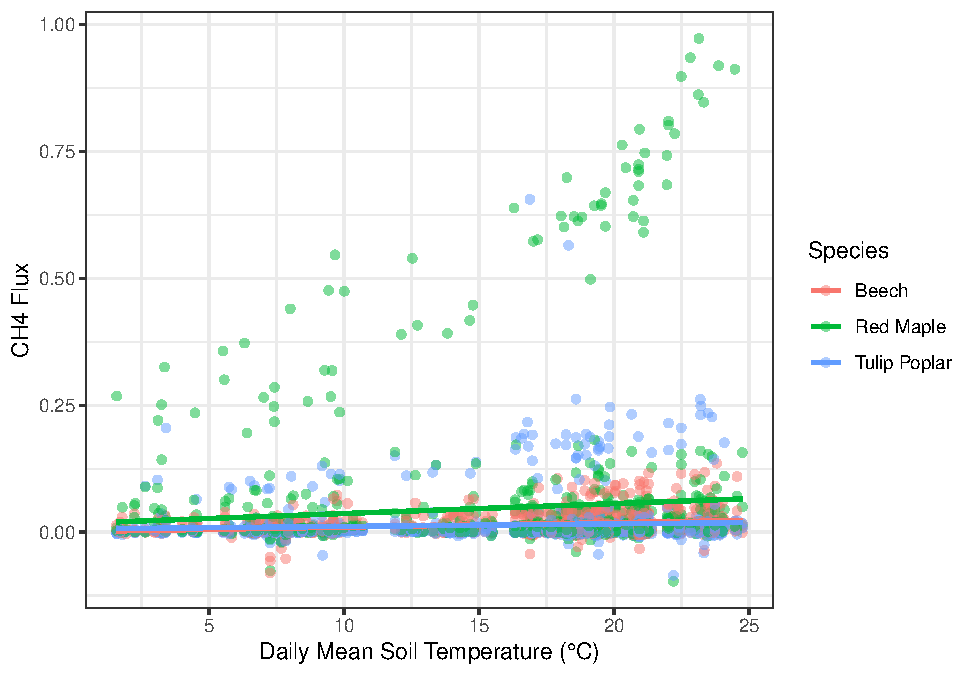
\includegraphics[keepaspectratio]{Mullen_TreeFlux_Analysis_files/Mullen_TreeFlux_Analysis_files/figure-latex/unnamed-chunk-21-1.pdf}}

\subsection{CO2 Tree Flux x Soil Temp (colored by
species)}\label{co2-tree-flux-x-soil-temp-colored-by-species}

\begin{Shaded}
\begin{Highlighting}[]
\FunctionTok{ggplot}\NormalTok{(my\_data,}\FunctionTok{aes}\NormalTok{(}\AttributeTok{x =}\NormalTok{ soil\_temp\_daily\_mean,}
                   \AttributeTok{y =}\NormalTok{ CO2\_lin\_flux.estimate,}
                   \AttributeTok{color =}\NormalTok{ Species)) }\SpecialCharTok{+}
\FunctionTok{geom\_point}\NormalTok{(}\AttributeTok{alpha =} \FloatTok{0.5}\NormalTok{) }\SpecialCharTok{+} \FunctionTok{geom\_smooth}\NormalTok{(}\AttributeTok{method =} \StringTok{"lm"}\NormalTok{, }\AttributeTok{se =} \ConstantTok{FALSE}\NormalTok{)}
\end{Highlighting}
\end{Shaded}

\begin{verbatim}
## `geom_smooth()` using formula = 'y ~ x'
\end{verbatim}

\pandocbounded{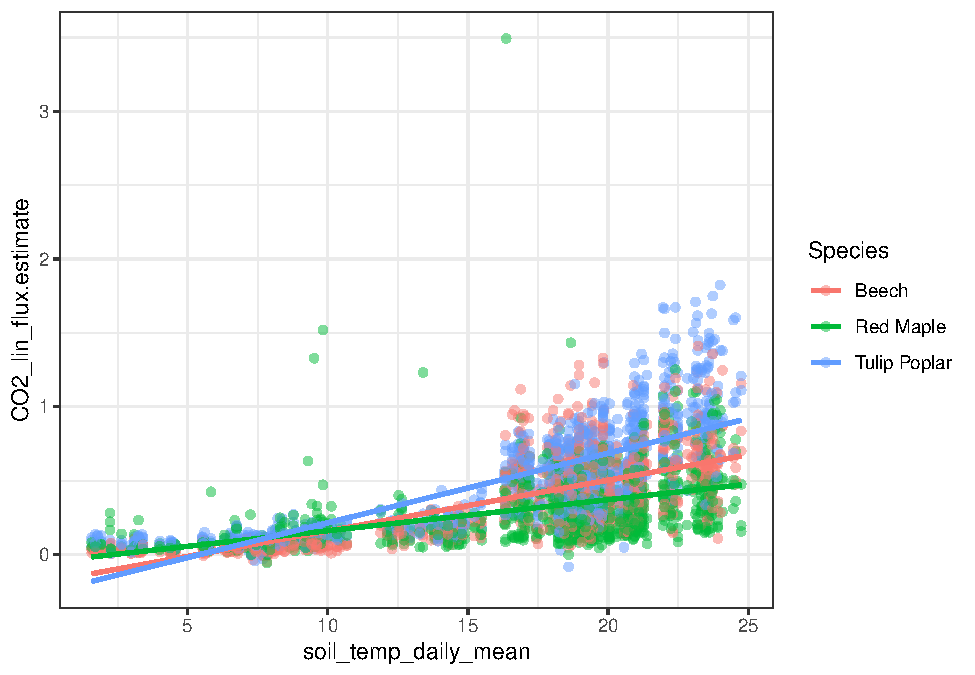
\includegraphics[keepaspectratio]{Mullen_TreeFlux_Analysis_files/Mullen_TreeFlux_Analysis_files/figure-latex/unnamed-chunk-22-1.pdf}}

\subsection{Methane and Soil Temp Over
Time}\label{methane-and-soil-temp-over-time}

\begin{Shaded}
\begin{Highlighting}[]
\FunctionTok{ggplot}\NormalTok{(my\_data, }\FunctionTok{aes}\NormalTok{(}\AttributeTok{x =}\NormalTok{ Date)) }\SpecialCharTok{+}
 \FunctionTok{geom\_line}\NormalTok{(}\FunctionTok{aes}\NormalTok{(}\AttributeTok{y =}\NormalTok{ CH4\_lin\_flux.estimate, }\AttributeTok{color =} \StringTok{"CH4"}\NormalTok{), }\AttributeTok{alpha =} \FloatTok{0.5}\NormalTok{) }\SpecialCharTok{+}
\FunctionTok{geom\_line}\NormalTok{(}\FunctionTok{aes}\NormalTok{(}\AttributeTok{y =}\NormalTok{ soil\_temp\_daily\_mean, }\AttributeTok{color =} \StringTok{"Soil Temp"}\NormalTok{), }\AttributeTok{alpha =} \FloatTok{0.7}\NormalTok{) }\SpecialCharTok{+}
 \FunctionTok{facet\_wrap}\NormalTok{(}\SpecialCharTok{\textasciitilde{}}\NormalTok{ Species) }\SpecialCharTok{+}
 \FunctionTok{scale\_color\_manual}\NormalTok{(}\AttributeTok{values =} \FunctionTok{c}\NormalTok{(}\StringTok{"CH4"} \OtherTok{=} \StringTok{"darkgreen"}\NormalTok{, }\StringTok{"Soil Temp"} \OtherTok{=} \StringTok{"red"}\NormalTok{)) }\SpecialCharTok{+}
\FunctionTok{labs}\NormalTok{( }\AttributeTok{title =} \StringTok{"CH4 Flux and Soil Temperature Over Time"}\NormalTok{,}
     \AttributeTok{y =} \StringTok{"Value (different scales)"}\NormalTok{,}
   \AttributeTok{color =} \StringTok{"Variable"}\NormalTok{    )}
\end{Highlighting}
\end{Shaded}

\pandocbounded{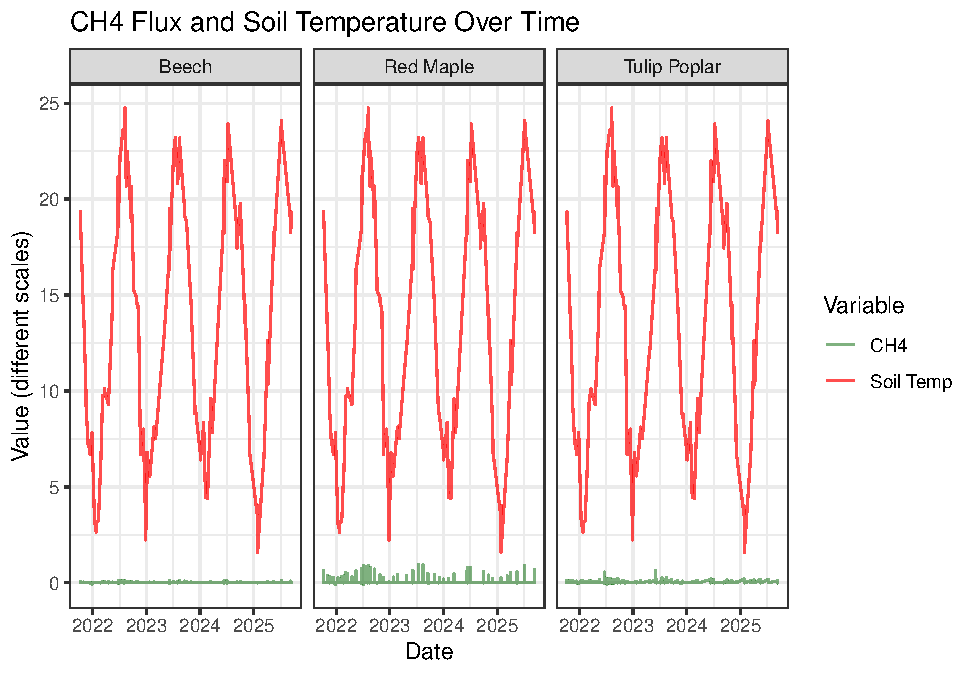
\includegraphics[keepaspectratio]{Mullen_TreeFlux_Analysis_files/Mullen_TreeFlux_Analysis_files/figure-latex/unnamed-chunk-23-1.pdf}}

\subsection{Methane vs Soil Temp (by
plot)}\label{methane-vs-soil-temp-by-plot}

\begin{Shaded}
\begin{Highlighting}[]
\FunctionTok{ggplot}\NormalTok{(my\_data, }\FunctionTok{aes}\NormalTok{(}\AttributeTok{x =}\NormalTok{ soil\_temp\_daily\_mean, }\AttributeTok{y =}\NormalTok{ CH4\_lin\_flux.estimate)) }\SpecialCharTok{+}
   \FunctionTok{geom\_point}\NormalTok{(}\FunctionTok{aes}\NormalTok{(}\AttributeTok{color =}\NormalTok{ Plot), }\AttributeTok{alpha =} \FloatTok{0.5}\NormalTok{) }\SpecialCharTok{+}
       \FunctionTok{geom\_smooth}\NormalTok{(}\AttributeTok{method =} \StringTok{"lm"}\NormalTok{, }\AttributeTok{se =} \ConstantTok{FALSE}\NormalTok{) }\SpecialCharTok{+}
     \FunctionTok{facet\_wrap}\NormalTok{(}\SpecialCharTok{\textasciitilde{}}\NormalTok{ Species) }\SpecialCharTok{+}
    \FunctionTok{geom\_vline}\NormalTok{(}\AttributeTok{data =}\NormalTok{ flood\_date,}
\FunctionTok{aes}\NormalTok{(}\AttributeTok{xintercept =} \ConstantTok{NA}\NormalTok{), }\AttributeTok{linetype =} \StringTok{"dashed"}\NormalTok{)  }\CommentTok{\# placeholder style}
\end{Highlighting}
\end{Shaded}

\begin{verbatim}
## `geom_smooth()` using formula = 'y ~ x'
\end{verbatim}

\begin{verbatim}
## Warning: Removed 9 rows containing missing values or values outside the scale range
## (`geom_vline()`).
\end{verbatim}

\pandocbounded{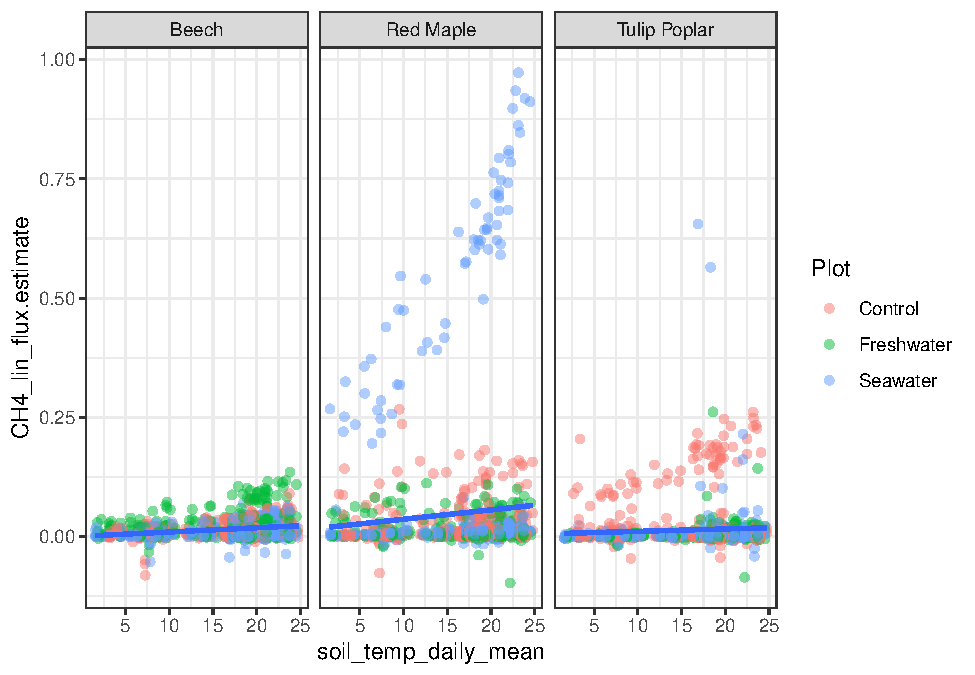
\includegraphics[keepaspectratio]{Mullen_TreeFlux_Analysis_files/Mullen_TreeFlux_Analysis_files/figure-latex/unnamed-chunk-24-1.pdf}}

\subsection{Soil Temperature × Treatment Effects on CH4
Flux}\label{soil-temperature-treatment-effects-on-ch4-flux}

\begin{Shaded}
\begin{Highlighting}[]
\FunctionTok{ggplot}\NormalTok{(my\_data, }\FunctionTok{aes}\NormalTok{(}\AttributeTok{x =}\NormalTok{ soil\_temp\_daily\_mean,}
                  \AttributeTok{y =}\NormalTok{ CH4\_lin\_flux.estimate,}
                     \AttributeTok{color =}\NormalTok{ Plot)) }\SpecialCharTok{+}
     \FunctionTok{geom\_point}\NormalTok{(}\AttributeTok{alpha =} \FloatTok{0.4}\NormalTok{) }\SpecialCharTok{+}
     \FunctionTok{geom\_smooth}\NormalTok{(}\AttributeTok{method =} \StringTok{"lm"}\NormalTok{, }\AttributeTok{se =} \ConstantTok{FALSE}\NormalTok{) }\SpecialCharTok{+}
     \FunctionTok{facet\_wrap}\NormalTok{(}\SpecialCharTok{\textasciitilde{}}\NormalTok{ Species) }\SpecialCharTok{+}
     \FunctionTok{labs}\NormalTok{(}\AttributeTok{title =} \StringTok{"Soil Temperature × Treatment Effects on CH4 Flux"}\NormalTok{)}
\end{Highlighting}
\end{Shaded}

\begin{verbatim}
## `geom_smooth()` using formula = 'y ~ x'
\end{verbatim}

\pandocbounded{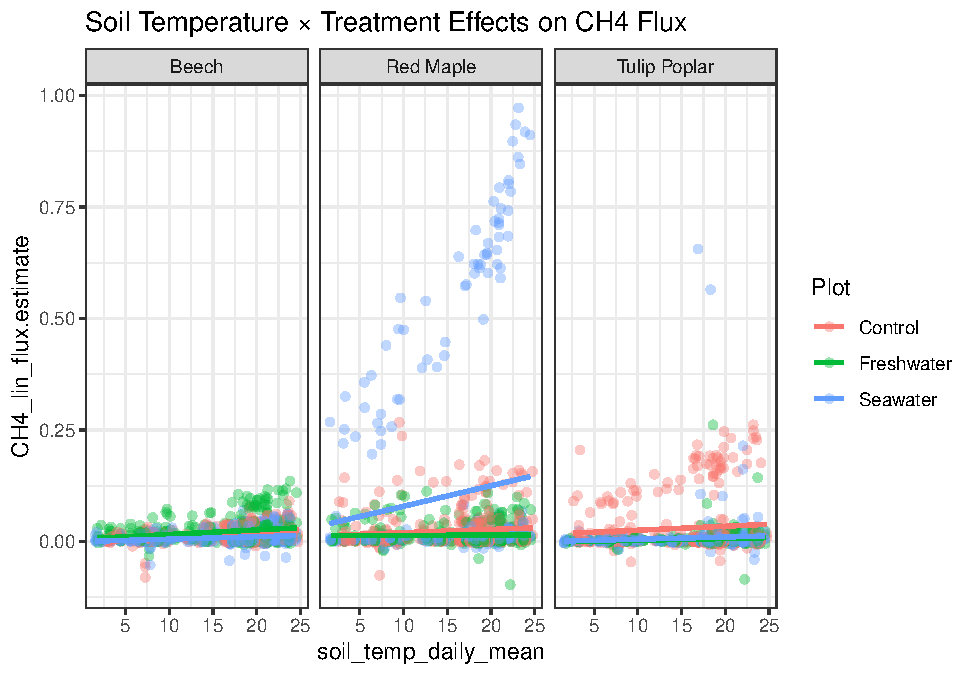
\includegraphics[keepaspectratio]{Mullen_TreeFlux_Analysis_files/Mullen_TreeFlux_Analysis_files/figure-latex/unnamed-chunk-25-1.pdf}}

\subsection{Methane vs Soil Temp (by
plot)}\label{methane-vs-soil-temp-by-plot-1}

\begin{Shaded}
\begin{Highlighting}[]
\FunctionTok{ggplot}\NormalTok{(my\_data, }\FunctionTok{aes}\NormalTok{(}\AttributeTok{x =}\NormalTok{ soil\_temp\_daily\_mean, }\AttributeTok{y =}\NormalTok{ CH4\_lin\_flux.estimate)) }\SpecialCharTok{+}
 \FunctionTok{geom\_point}\NormalTok{(}\FunctionTok{aes}\NormalTok{(}\AttributeTok{color =}\NormalTok{ Plot), }\AttributeTok{alpha =} \FloatTok{0.5}\NormalTok{) }\SpecialCharTok{+}
      \FunctionTok{geom\_smooth}\NormalTok{(}\AttributeTok{method =} \StringTok{"lm"}\NormalTok{, }\AttributeTok{se =} \ConstantTok{FALSE}\NormalTok{, }\AttributeTok{color =} \StringTok{"black"}\NormalTok{) }\SpecialCharTok{+}
      \FunctionTok{facet\_wrap}\NormalTok{(}\SpecialCharTok{\textasciitilde{}}\NormalTok{ Species) }\SpecialCharTok{+}
      \FunctionTok{labs}\NormalTok{(}
          \AttributeTok{title =} \StringTok{"CH4 Flux vs Soil Temperature"}\NormalTok{,}
\AttributeTok{x =} \StringTok{"Soil Temperature (°C)"}\NormalTok{,}
 \AttributeTok{y =} \StringTok{"CH4 Flux"}\NormalTok{     )}
\end{Highlighting}
\end{Shaded}

\begin{verbatim}
## `geom_smooth()` using formula = 'y ~ x'
\end{verbatim}

\pandocbounded{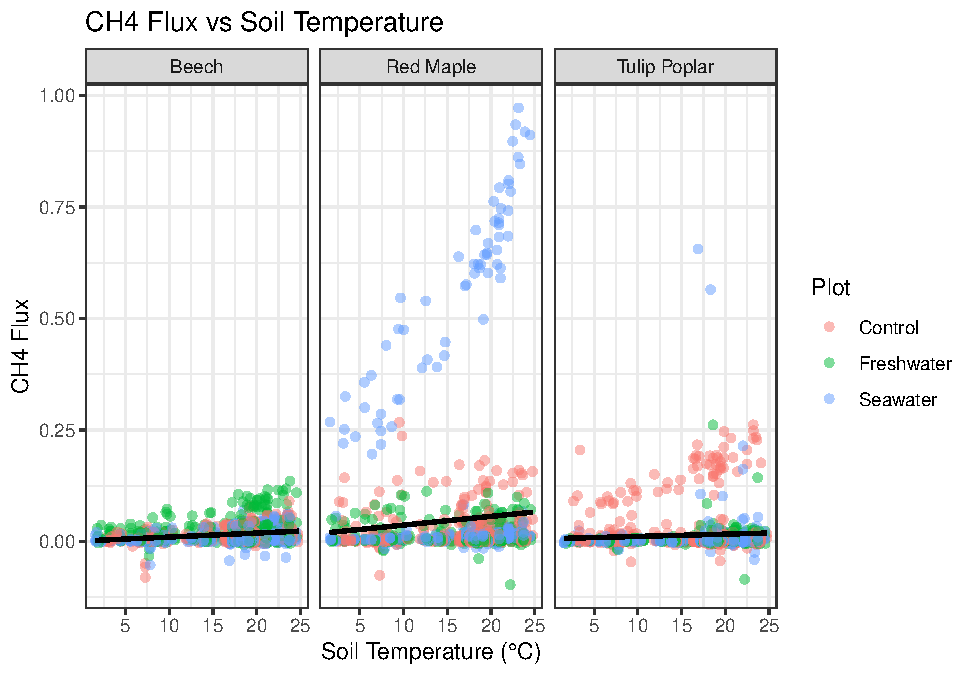
\includegraphics[keepaspectratio]{Mullen_TreeFlux_Analysis_files/Mullen_TreeFlux_Analysis_files/figure-latex/unnamed-chunk-26-1.pdf}}

\subsection{Nonlinear Temperature Response of CH4 (What is the actual
shape of the temperature--methane
relationship?)}\label{nonlinear-temperature-response-of-ch4-what-is-the-actual-shape-of-the-temperaturemethane-relationship}

\subsubsection{Locally Estimated Scatterplot Smoothing =
LOESS}\label{locally-estimated-scatterplot-smoothing-loess}

\begin{Shaded}
\begin{Highlighting}[]
\FunctionTok{ggplot}\NormalTok{(my\_data, }\FunctionTok{aes}\NormalTok{(soil\_temp\_daily\_mean, CH4\_lin\_flux.estimate)) }\SpecialCharTok{+}
  \FunctionTok{geom\_point}\NormalTok{(}\AttributeTok{alpha =} \FloatTok{0.4}\NormalTok{, }\FunctionTok{aes}\NormalTok{(}\AttributeTok{color =}\NormalTok{ Species)) }\SpecialCharTok{+}
  \FunctionTok{geom\_smooth}\NormalTok{(}\AttributeTok{method =} \StringTok{"loess"}\NormalTok{, }\AttributeTok{se =} \ConstantTok{FALSE}\NormalTok{) }\SpecialCharTok{+}
  \FunctionTok{facet\_wrap}\NormalTok{(}\SpecialCharTok{\textasciitilde{}}\NormalTok{ Plot) }\SpecialCharTok{+}
  \FunctionTok{labs}\NormalTok{(}\AttributeTok{title =} \StringTok{"Nonlinear Temperature Response of CH4"}\NormalTok{)}
\end{Highlighting}
\end{Shaded}

\begin{verbatim}
## `geom_smooth()` using formula = 'y ~ x'
\end{verbatim}

\pandocbounded{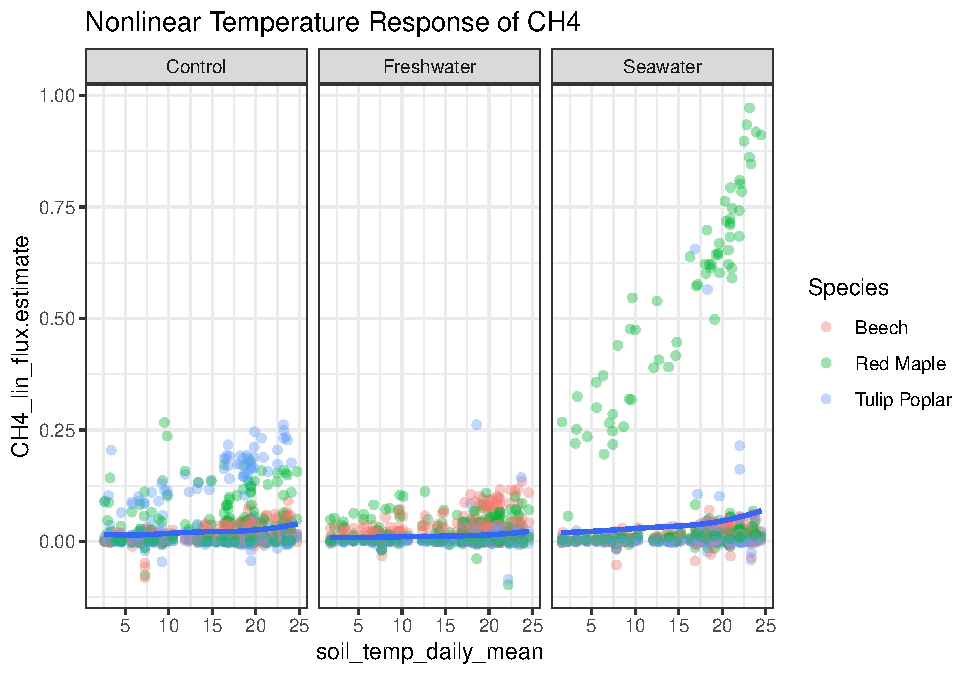
\includegraphics[keepaspectratio]{Mullen_TreeFlux_Analysis_files/Mullen_TreeFlux_Analysis_files/figure-latex/unnamed-chunk-27-1.pdf}}

\subsection{Species Differences in Temperature Sensitivity (Do different
species have different average rates of response to
temperature?)}\label{species-differences-in-temperature-sensitivity-do-different-species-have-different-average-rates-of-response-to-temperature}

\begin{Shaded}
\begin{Highlighting}[]
\FunctionTok{ggplot}\NormalTok{(my\_data, }\FunctionTok{aes}\NormalTok{(soil\_temp\_daily\_mean,}
\NormalTok{                    CH4\_lin\_flux.estimate,}
                    \AttributeTok{color =}\NormalTok{ Species)) }\SpecialCharTok{+}
  \FunctionTok{geom\_point}\NormalTok{(}\AttributeTok{alpha =} \FloatTok{0.4}\NormalTok{) }\SpecialCharTok{+}
  \FunctionTok{geom\_smooth}\NormalTok{(}\AttributeTok{method =} \StringTok{"lm"}\NormalTok{, }\AttributeTok{se =} \ConstantTok{FALSE}\NormalTok{) }\SpecialCharTok{+}
  \FunctionTok{labs}\NormalTok{(}\AttributeTok{title =} \StringTok{"Species Differences in Temperature Sensitivity"}\NormalTok{)}
\end{Highlighting}
\end{Shaded}

\begin{verbatim}
## `geom_smooth()` using formula = 'y ~ x'
\end{verbatim}

\pandocbounded{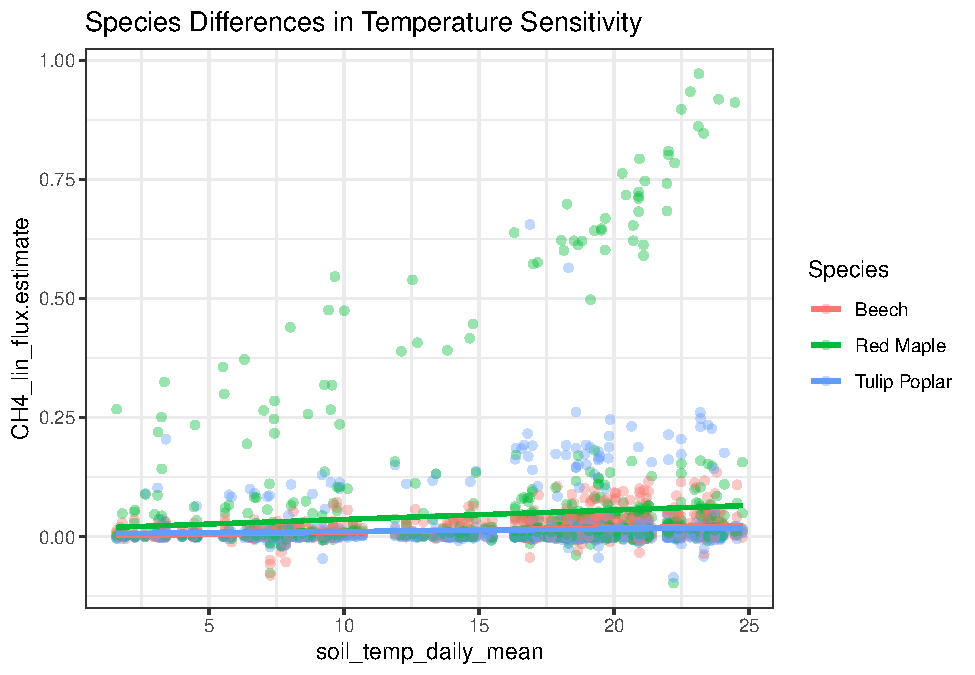
\includegraphics[keepaspectratio]{Mullen_TreeFlux_Analysis_files/Mullen_TreeFlux_Analysis_files/figure-latex/unnamed-chunk-28-1.pdf}}

\end{document}
